\documentclass{article}

%**************************************************************
% Importazione package
%**************************************************************

% permette di modificare i margini
%\usepackage[top=3.1cm, bottom=3.1cm, left=2.2cm, right=2.2cm]{geometry}
\usepackage[a4paper]{geometry}

% necessario per risolvere il problema del carattere invisibile per l'a capo
% \DeclareUnicodeCharacter{00A0}{ }

% per scrivere in italiano e in inglese;
% l'ultima lingua (l'italiano) risulta predefinita
\usepackage[english, italian]{babel}

% imposta lo stile italiano per i paragrafi
\usepackage{parskip}

% fornice elenchi numerati in ordine inverso
\usepackage{etaremune}

% comandi per l'appendice
\usepackage{appendix}
\renewcommand\appendixtocname{Appendici}
\renewcommand{\appendixpagename}{Appendici}

% numera anche i paragrafi
\setcounter{secnumdepth}{6}

% elenca anche i paragrafi nell'indice
\setcounter{tocdepth}{6}

% permetti di definire dei colori
\usepackage[usenames,dvipsnames]{color}

% permette di inserire le immagini/tabelle esattamente dove viene usato il
% comando \begin{figure}[H] ... \end{figure}
% evitando che venga spostato in automatico
\usepackage{float}

% permette l'inserimento di url e di altri tipi di collegamento
\usepackage[colorlinks=true]{hyperref}

\hypersetup{
    colorlinks=true, % false: boxed links; true: colored links
    citecolor=black,
    filecolor=black,
    linkcolor=black, % color of internal links
    urlcolor=Maroon  % color of external links
}

% immagini
\usepackage{graphicx}

% permette di riferirsi all'ultima pagina con \pageref{LastPage}
\usepackage{lastpage}

% tabelle su più pagine
\usepackage{longtable}

% per avere dei comandi in più da poter usare sulle tabelle
\usepackage{booktabs}

% tabelle con il campo X per riempire lo spazio rimanente sulla riga
\usepackage{tabularx}

% multirow per tabelle
\usepackage{multirow}

% colore di sfondo per le celle
\usepackage[table]{xcolor}
%\rowcolors{2}{gray!25}{} % Colora righe alterne in grigio (non funziona bene)

% permette di fare longtable larghe tutta la pagina (parametro x)
% su Ubuntu non si può installare il pacchetto, deve essere in model/
\usepackage{tabu}

% imposta lo spazio tra le righe di una tabella
\setlength{\tabulinesep}{6pt}

% definisci un nuovo tipo di colonna P che permette di andare a capo con \newline
% e giustificata a sinistra
\usepackage{array}
\usepackage{ragged2e}
\newcolumntype{P}[1]{>{\RaggedRight \hspace{0pt}}m{#1}}

% personalizza l'intestazione e piè di pagina
\usepackage{fancyhdr}

% permette di inserire caratteri speciali
\usepackage{textcomp}

% permette di aggiustare i margini e centrare tabelle e figure
\usepackage{changepage}

%Permette di includere i grafici a barre
%IMPORTANTE: deve essere caricato prima di /pgfgantt altrimenti causa conflitto
\usepackage{pgfplots}

% permette di includere i diagrammi Gantt
% su Ubuntu non si può installare il pacchetto, deve essere in model/
\usepackage{pgfgantt}

% permette di includere i grafici a torta
\usepackage{pgf-pie}

% necessario per pgf-pie
\usepackage{tikz}

% permette i path delle immagini con gli spazi
\usepackage{grffile}

% ruota le immagini
\usepackage{rotating}

% permetti di calcolare le larghezze facendo calcoli
\usepackage{calc}


%%
%% Definizione di path globali
%%
% Path assoluta a questa directory, va passato come argomento il resto della path
\newcommand{\ModelPath}[1]{/data/sources/model/#1}

% Path per accedere a modelassets
\newcommand{\ModelAssets}[1]{\ModelPath{modelassets}/#1}

% Path globali per la ricerca di immagini
\graphicspath{
	{/data/logo/PNG}
	{/data/logo/Square}
}



\fancypagestyle{plain}{
	% cancella tutti i campi di intestazione e piè di pagina
	\fancyhf{}
	\lhead{
		
\includegraphics[width=1.5cm, keepaspectratio=true]{argo_icona.png}
		\parbox[b]{5cm}{
			\emph{\GroupName{}} \vspace{0pt} \\
			\emph{Progetto \ProjectName{}} \vspace{0pt}
		}
	}
	\chead{}


	\lfoot{
		\DocTitle{} \\
		% differenzia a seconda che \DocVersion{} stampi testo o no
		\setbox0=\hbox{\DocVersion{}\unskip}\ifdim\wd0=0pt
			% nulla
		\else
			v \DocVersion{}
		\fi
	}
	\rfoot{\thepage{} di \pageref{LastPage}}

	% Visualizza una linea orizzontale in cima e in fondo alla pagina
	\renewcommand{\headrulewidth}{0.3pt}
	\renewcommand{\footrulewidth}{0.3pt}
}
\setlength{\headheight}{30pt}
\pagestyle{plain}

% allarga l'header a tutta la pagina
%\fancyhfoffset[L]{\oddsidemargin + \hoffset + 1in}
%\fancyhfoffset[R]{\evensidemargin + \marginparwidth - \marginparsep}

% Per inserire del codice sorgente formattato
\usepackage{listings}
\definecolor{darkgray}{rgb}{.4,.4,.4}
\definecolor{purple}{rgb}{0.65, 0.12, 0.82}
\definecolor{mygreen}{rgb}{0,0.6,0}
\definecolor{mygray}{rgb}{0.5,0.5,0.5}
\definecolor{mymauve}{rgb}{0.58,0,0.82}

\lstset{
  extendedchars=true,          % lets you use non-ASCII characters
  inputencoding=utf8,   % converte i caratteri utf8 in latin1, richiede \usepackage{listingsutf8} anzichè listings
  basicstyle=\ttfamily,        % the size of the fonts that are used for the code
  breakatwhitespace=false,     % sets if automatic breaks should only happen at whitespace
  breaklines=true,             % sets automatic line breaking
  captionpos=b,                % sets the caption-position to top
  commentstyle=\color{mygreen},   % comment style
  frame=none,               % adds a frame around the code
  keepspaces=true,            % keeps spaces in text, useful for keeping indentation of code (possibly needs columns=flexible)
  keywordstyle=\color{blue}\bfseries,     % keyword style
  numbers=none,               % where to put the line-numbers; possible values are (none, left, right)
  numbersep=5pt,              % how far the line-numbers are from the code
  numberstyle=\color{mygray}, % the style that is used for the line-numbers
  rulecolor=\color{black},    % if not set, the frame-color may be changed on line-breaks within not-black text (e.g. comments (green here))
  showspaces=false,           % show spaces everywhere adding particular underscores; it overrides 'showstringspaces'
  showstringspaces=false,     % underline spaces within strings only
  showtabs=false,             % show tabs within strings adding particular underscores
  stepnumber=5,               % the step between two line-numbers. If it's 1, each line will be numbered
  stringstyle=\color{red},    % string literal style
  tabsize=4,                  % sets default tabsize
  firstnumber=1      % visualizza i numeri dalla prima linea
}

% Permetti di utilizzare il grassetto per i caratteri Typewriter (per es. il font di \code{...} e \file{...})
\usepackage[T1]{fontenc}
\usepackage{lmodern}

% Permette di resettare il contatore delle note a piè di pagina ad ogni pagina
\usepackage[perpage, bottom, stable]{footmisc}
\patchcmd{\footref}{\ref}{\ref*}{}{}

% Per poter usare il carattere ° (anche nelle formule matematiche)
\usepackage{gensymb}
\usepackage{newunicodechar}
\newunicodechar{°}{\degree}

% Per importare svg
\usepackage{svg}
%\setsvg{inkscape = inkscape -z -D}

% Per numerare le tabelle e le figure con la sezione in cui si trovano
\usepackage{amsmath}
\numberwithin{figure}{section}
\numberwithin{table}{section}

% Per aggiungere un nuovo lovello di profondita (subsubparagraph)

\makeatletter
\newcounter{subsubparagraph}[subparagraph]
\renewcommand\thesubsubparagraph{%
	\thesubparagraph.\@arabic\c@subsubparagraph}
\newcommand\subsubparagraph{%
	\@startsection{subsubparagraph}    % counter
	{6}                              % level
	{\parindent}                     % indent
	{3.25ex \@plus 1ex \@minus .2ex} % beforeskip
	{-1em}                           % afterskip
	{\normalfont\normalsize\bfseries}}
\newcommand\l@subsubparagraph{\@dottedtocline{6}{12em}{5em}}
\newcommand{\subsubparagraphmark}[1]{}
\def\endsubsubparagraph{\par
	\if@noskipsec
	\ifx\@svsechd\@undefined\else\leavevmode\fi
	\fi}
\makeatletter
\def\toclevel@subsubparagraph{6}
\makeatother
% Use \ul{arg} to undlerline text
\usepackage{soul}

% Per le pagine in orientamento orizzontale
\usepackage{pdflscape}
\usepackage{afterpage}

% Set vertical space in tables
\def\arraystretch{1.5}

% Modifica font
\usepackage{fontspec}

\setmainfont{Poppins}[
    Path=\ModelAssets{poppins/} ,
    Extension = .otf ,
    UprightFont=*-Regular ,
    BoldFont=*-Bold ,
    ItalicFont=*-Italic ,
    BoldItalicFont=*-BoldItalic
]
%%%%%%%%%%%%%%
%  COSTANTI  %
%%%%%%%%%%%%%%

% In questa prima parte vanno definite le 'costanti' utilizzate da due o più documenti.

% Serve a dare la giusta formattazione alle parole presenti nel glossario
% il nome del comando \glossary è già usato da LaTeX
% permette di distingure la prima occorrenza della parola nel documento
\usepackage{xparse}
\ExplSyntaxOn
\seq_new:N \l_hernan_seq
\NewDocumentCommand{\glossario}{m}{
    \seq_if_in:NnTF{\l_hernan_seq}{#1}{
      \textit{#1\ped{\ped{G}}}
    }{
      \seq_put_left:Nn{\l_hernan_seq}{#1}
      \textit{#1\ped{\ped{G}}}
    }
}
\ExplSyntaxOff

% Meglio non mettere gli \emph dentro le costanti, in certi casi creano problemi
\newcommand{\GroupName}{Argo}
\newcommand{\GroupEmail}{argo.unipd@gmail.com}
\newcommand{\ProjectName}{ChatSQL}
\newcommand{\ProjectVersion}{}

\newcommand{\Proponente}{Zucchetti S.p.A.}
\newcommand{\Committente}{Prof. Tullio Vardanega \\ Prof. Riccardo Cardin}
\newcommand{\CommittenteInline}{Prof. Tullio Vardanega, Prof. Riccardo Cardin}
\newcommand{\ResponsabileInCarica}{\mattia}

% La versione dei documenti deve essere definita qui in global, perchè serve anche agli altri documenti
\newcommand{\VersioneNP}{1.0.1}  % Norme di Progetto
\newcommand{\VersioneAR}{1.0.2}  % Analisi dei Requisiti
\newcommand{\VersionePQ}{1.0.3}  % Piano di Qualifica
\newcommand{\VersioneG}{1.0.1}   % Glossario
\newcommand{\VersionePP}{1.0.4}  % Piano di Progetto
\newcommand{\VersioneST}{0.0.7} % Specifica Tecnica
\newcommand{\VersioneMU}{0.0.6} % Manuale Utente

% Il verbale non ha versionamento.
% Lasciare vuoto, non mettere trattini o puntini
% Non sono permessi numeri nel nome di un comando :(
\newcommand{\VersioneVprimo}{}
\newcommand{\VersioneVsecondo}{}

% Per riferirsi ad alti documenti globalmente, se la versione nella parte soprastante è vuota il numero non compare
\newcommand{\PianoDiProgetto}{\emph{Piano di Progetto v\VersionePP{}}}
\newcommand{\NormeDiProgetto}{\emph{Norme di Progetto v\VersioneNP{}}}
\newcommand{\PianoDiQualifica}{\emph{Piano di Qualifica v\VersionePQ{}}}
\newcommand{\AnalisiDeiRequisiti}{\emph{Analisi dei Requisiti v\VersioneAR{}}}
\newcommand{\Glossario}{\emph{Glossario v\VersioneG{}}}
\newcommand{\SpecificaTecnica}{\emph{Specifica Tecnica v\VersioneST{}}}
\newcommand{\ManualeUtente}{\emph{Manuale Utente v\VersioneMU{}}}

% Per riferirsi alle revisioni usare i comandi seguenti:
\newcommand{\RTB}{Requirements and Technology Baseline}
\newcommand{\PB}{Product Baseline}
\newcommand{\CA}{Customer Acceptance}

% Comandi utili per riferirsi alle varie fasi
\newcommand{\AReq}{Analisi dei Requisiti}
\newcommand{\ARischi}{Analisi dei rischi}
\newcommand{\AD}{Analisi di Dettaglio}
\newcommand{\PA}{Progettazione Architetturale}
\newcommand{\PD}{Progettazione di Dettaglio}
\newcommand{\Cod}{Codifica}
\newcommand{\VV}{Verifica e Validazione}

%Comandi shortcut per riferirsi a documenti SENZA versione
\newcommand{\PdP}{\emph{Piano di Progetto}}
\newcommand{\PdQ}{\emph{Piano di Qualifica}}
\newcommand{\NdP}{\emph{Norme di Progetto}}
\newcommand{\AdR}{\emph{Analisi dei Requisiti}}
\newcommand{\Gls}{\emph{Glossario}}
\newcommand{\ST}{\emph{Specifica Tecnica}}
\newcommand{\MU}{\emph{Manuale Utente}}

%Comando shortcut per riferirsi al Way of Working
\newcommand{\WoW}{Way of Working}

% Comandi utili per riferirsi ai componenti del gruppo (Diari delle modifiche)
\newcommand{\tommaso}{Tommaso Stocco}
\newcommand{\sebastiano}{Sebastiano Lewental}
\newcommand{\marco}{Marco Cristo}
\newcommand{\riccardo}{Riccardo Cavalli}
\newcommand{\raul}{Raul Pianon}
\newcommand{\martina}{Martina Dall'Amico}
\newcommand{\mattia}{Mattia Zecchinato}


% Comandi utili per riferirsi ai ruoli di progetto
%% non rimuovere i caratteri % gestiscono gli spazi
\NewDocumentCommand{\Responsabile}{o}{%
  \IfNoValueTF{#1}
    {\textit{responsabile di progetto}}
    {\textit{Responsabile di progetto}}%
}
\NewDocumentCommand{\Amministratore}{o}{%
  \IfNoValueTF{#1}
    {\textit{amministratore}}
    {\textit{Amministratore}}%
}
\NewDocumentCommand{\Analista}{o}{%
  \IfNoValueTF{#1}
    {\textit{analista}}
    {\textit{Analista}}%
}
\NewDocumentCommand{\Progettista}{o}{%
  \IfNoValueTF{#1}
    {\textit{progettista}}
    {\textit{Progettista}}%
}
\NewDocumentCommand{\Programmatore}{o}{%
  \IfNoValueTF{#1}
    {\textit{programmatore}}
    {\textit{Programmatore}}%
}
\NewDocumentCommand{\Verificatore}{o}{%
  \IfNoValueTF{#1}
    {\textit{verificatore}}
    {\textit{Verificatore}}%
}
\NewDocumentCommand{\Redattore}{o}{%
  \IfNoValueTF{#1}
    {\textit{redattore}}
    {\textit{Redattore}}%
}

\NewDocumentCommand{\Amministratrice}{o}{%
  \IfNoValueTF{#1}
    {\textit{amministratrice}}
    {\textit{Amministratrice}}%
}
\NewDocumentCommand{\Programmatrice}{o}{%
  \IfNoValueTF{#1}
    {\textit{programmatrice}}
    {\textit{Programmatrice}}%
}
\NewDocumentCommand{\Redattrice}{o}{%
  \IfNoValueTF{#1}
    {\textit{redattrice}}
    {\textit{Redattrice}}%
}

% FIXME: rimuovere
% \newcommand{\Responsabile}{\textit{responsabile di progetto}}
% \newcommand{\Amministratore}{\textit{amministratore}}
% \newcommand{\Analista}{\textit{analista}}
% \newcommand{\Progettista}{\textit{progettista}}
% \newcommand{\Programmatore}{\textit{programmatore}}
% \newcommand{\Verificatore}{\textit{verificatore}}
% \newcommand{\Redattore}{\textit{redattore}}

% \newcommand{\Amministratrice}{\textit{amministratrice}}
% \newcommand{\Programmatrice}{\textit{programmatrice}}
% \newcommand{\Redattrice}{\textit{redattrice}}


\newcommand{\ScopoDelProdotto}{}

\newcommand{\ScopoDelProdottoEng}{}

\newcommand{\GlossarioIntroduzione}{
  Allo scopo di evitare incomprensioni relative al linguaggio utilizzato nella documentazione di progetto, viene fornito un \Gls, nel quale ciascun termine è corredato da una spiegazione che mira a disambiguare il suo significato. I termini tecnici, gli acronimi e i vocaboli ritenuti ambigui vengono formattati in corsivo all'interno dei rispettivi documenti e marcati con una lettera \ped{G} in pedice. Tutte le ricorrenze di un termine definito nel \Gls\ subiscono la formattazione sopracitata.
}

%Comando per i verbali esterni (solamente quando ci sono tanti termini tecnici o ambigui)
\newcommand{\GlossarioIntroduzioneVE}{
  Allo scopo di evitare incomprensioni relative al linguaggio utilizzato nella documentazione di progetto, viene fornito un \Gls, nel quale ciascun termine è corredato da una spiegazione che mira a disambiguare il suo significato. I termini tecnici, gli acronimi e i vocaboli ritenuti ambigui vengono formattati in corsivo all'interno dei rispettivi documenti e marcati con una lettera \ped{G} in pedice. In questo documento viene formattata solamente la prima ricorrenza di un termine definito nel \Gls.
}

\newcommand{\ToBeContinued}{\textit{Continua nella prossima pagina}}

% Altri comandi utili
\newcommand{\email}{email}
\newcommand*{\sezione}[1]{\hyperref[{#1}]{sezione §\ref*{#1}}}
\newcommand*{\appendice}[1]{\hyperref[{#1}]{Appendice \autoref*{#1}}}

% Bisognerebbe aggiungere anche altri brand utilizzati spesso nei vari documenti
\newcommand{\Macos}{macOs}

%%%%%%%%%%%%%%
%  FUNZIONI  %
%%%%%%%%%%%%%%

% In questa seconda parte vanno definite le 'funzioni' utilizzate da due o più documenti.

% Comando per usare comodamente le virgolette
\newcommand{\virgolette}[1]{``#1''}

\newcommand\flextt{%
	\fontdimen2\font=0.2em% interword space
	\fontdimen3\font=0.1em% interword stretch
	\fontdimen4\font=0.1em% interword shrink
	\fontdimen7\font=0.2em% extra space
	\hyphenchar\font=`\-
}

% Serve a dare la giusta formattazione al codice inline
\newcommand{\code}[1]{\ttfamily\flextt{#1}\normalfont}

% Serve a dare la giusta formattazione a tutte le path presenti nei documenti
\newcommand{\file}[1]{\flextt{#1}}

% Permette di andare a capo all'interno di una cella in una tabella
\newcommand{\multiLineCell}[2][c]{\begin{tabular}[#1]{@{}l@{}}#2\end{tabular}}

% Per l'allineamento delle immagini
\usepackage[export]{adjustbox}

% Genera automaticamente la pagina di copertina
\newcommand{\makeFrontPage}{
  % Declare new goemetry for the title page only.
  \newgeometry{top=2cm}
  \begin{titlepage}
  \begin{center}
  \vspace*{2cm}
  \begin{center}
  
\includegraphics[width=8cm]{argo_square.png}
  \end{center}

%  \vspace{1cm}

  \begin{Huge}
  \textbf{\DocTitle{}}
  \end{Huge}

  \textbf{\emph{Gruppo \GroupName{} \, \texttwelveudash{} \, Progetto \ProjectName{}}}

  \vspace{10pt}

  \bgroup
  \def\arraystretch{1.3}
  \begin{tabular}{ r|l }
    \multicolumn{2}{c}{\textbf{Informazioni sul documento}} \\
    \hline
    \ifx\DocVersion\empty
      \ifdefined\DocData
        \ifx\DocData\empty
          % lascio vuoto
        \else
          \textbf{Data} & \DocData{} \\
        \fi
      \fi
    \else
      \textbf{Versione} & \faIcon{tag} \DocVersion{} \\
    \fi
    \textbf{Approvazione} & \multiLineCell[t]{\DocApprovazione{}} \\
    \textbf{Uso} & \DocUso{} \\
    \textbf{Distribuzione} & \multiLineCell[t]{\DocDistribuzione{}} \\
  \end{tabular}
  \egroup

  \vspace*{\fill}

  \begin{figure}[H]
	\includegraphics[height=3.5cm, center]{\ModelAssets{logo_unipd.png}}
  \end{figure}
  \end{center}
  \end{titlepage}

  % Ends the declared geometry for the titlepage
  \restoregeometry
}

%%%%%%%%%%%%%%
%  COSTANTI  %
%%%%%%%%%%%%%%

% In questa prima parte vanno definite le 'costanti' utilizzate soltanto da questo documento.
% Devono iniziare con una lettera maiuscola per distinguersi dalle funzioni.

\newcommand{\DocTitle}{Verbale Riunione 2024-05-02}
\newcommand{\DocVersion}{1.0.0}
\newcommand{\DocApprovazione}{\raul}
\newcommand{\DocUso}{Interno}
\newcommand{\DocDistribuzione}{
	\Committente{} \\
	Gruppo \GroupName{}
}

% La descrizione del documento
\newcommand{\DocDescription}{
	Durante l'incontro sono state discusse le attività svolte durante la settimana e sono stati presentati e discussi i punti per il diario di bordo del 3 maggio 2024. È stata inoltre inviata una mail alla Proponente e fissato un incontro per il 6 maggio 2024.
}

%%%%%%%%%%%%%%
%  FUNZIONI  %
%%%%%%%%%%%%%%

% In questa seconda parte vanno definite le 'funzioni' utilizzate soltanto da questo documento.

\makeatletter
\newcommand\subsubsubsection{\@startsection{paragraph}{4}{\z@}{-2.5ex\@plus -1ex \@minus -.25ex}{1.25ex \@plus .25ex}{\normalfont\normalsize\bfseries}}
\makeatother

\begin{document}

\makeFrontPage

\section*{Registro delle modifiche}

\bgroup
\begin{adjustwidth}{-0.5cm}{-0.5cm}
	% MAX 12.5cm
 	\begin{longtable}{|P{1cm}|P{2.2cm}|P{2.7cm}|P{2.7cm}|>{\arraybackslash}P{3.8cm}|}
	  \hline
		\textbf{Ver.} & \textbf{Data} & \textbf{Redazione} & \textbf{Verifica} & \textbf{Descrizione} \\ 
		\hline
		\endfirsthead

		\hline
		\textbf{Ver.} & \textbf{Data} & \textbf{Redazione} & \textbf{Verifica} & \textbf{Descrizione} \\ 
		\hline
		\endhead

		\hline
		\multicolumn{5}{|r|}{{Continua nella prossima pagina}} \\ 
		\hline
		\endfoot

		\hline
		\endlastfoot

		% IN ORDINE DALLA MODIFICA PIÙ RECENTE ALLA PIÙ VECCHIA
		0.0.1 & 2024-06-09 & \martina & \riccardo & Stesura del documento \\
	\end{longtable}
\end{adjustwidth}
\egroup
\clearpage

\tableofcontents
\clearpage
\renewcommand{\listtablename}{Elenco delle tabelle}
\listoftables
\clearpage
\renewcommand{\listfigurename}{Elenco delle figure}
\listoffigures
\clearpage  

\section{Introduzione}

\subsection{Scopo del documento}
Il presente documento si propone di offrire una trattazione esaustiva dei casi d'uso e dei \glossario{requisiti} del progetto "ChatSQL", seguendo gli \glossario{standard di qualità} dell'ingegneria del software. Tale analisi è stata condotta attraverso un'approfondita valutazione del \glossario{capitolato} C9 presentato dalla Proponente(G) Zucchetti S.p.A., integrata da una stretta collaborazione durante gli incontri dedicati.
L'obiettivo principale è definire con precisione le caratteristiche e le necessità della web application proposta, la quale verrà definita propriamente all'interno della sezione 2)[qua ci mettiamo un link].

\subsection{Scopo del prodotto}
L’utilizzo di strumenti di facilitazione basati sull’utilizzo di \glossario{Intelligenza Artificiale} si sta diffondendo in maniera esponenziale, e anche gli utenti non facenti parte dell’area IT (\glossario{Information Technology}) li utilizzano con sempre maggior frequenza per velocizzare le attività quotidiane. L’azienda Zucchetti ha proposto lo sviluppo di un’applicazione che tramite l’utilizzo di LLM (\glossario{Large Language Model}) consente la generazione di \glossario{prompt} ottimizzati all’interrogazione di modelli dati basati su \glossario{database SQL}. I \glossario{prompt} potranno essere poi proposti a servizi di LLM come ChatGPT per la generazione della \glossario{query} di interrogazione da eseguire sul database.
L'applicazione sarà implementata come una web application accessibile attraverso i principali browser come Chrome, Firefox, Edge e Safari. Gli utenti di tipo operatore potranno caricare, a seguito di autenticazione, nell’applicativo i modelli dati da poter utilizzare per la generazione dei \glossario{prompt}. Gli utenti finali potranno chiedere tramite linguaggio naturale la generazione del \glossario{prompt} basandosi su uno specifico modello di dati. Il \glossario{prompt} generato e passato ad un servizio di LLM genererà la \glossario{query} da poter eseguire.

\subsection{Glossario}
\GlossarioIntroduzione

\subsection{Riferimenti}
\subsubsection{Riferimenti normativi}
\begin{itemize}
  \item Capitolato C9 - ChatSQL:\\ \href{https://www.math.unipd.it/~tullio/IS-1/2023/Progetto/C9.pdf}{https://www.math.unipd.it/\~tullio/IS-1/2023/Progetto/C9.pdf} \\ \href{https://www.math.unipd.it/~tullio/IS-1/2023/Progetto/C9.pdf}{https://www.math.unipd.it/\~tullio/IS-1/2023/Progetto/C9p.pdf};
  \item Norme di Progetto:\\ \href{https://github.com/Argo-swe/argo-swe.github.io/blob/main/2_RTB/NormeDiProgetto.pdf}{https://github.com/Argo-swe/argo-swe.github.io/blob/main/2\_RTB/ \\ NormeDiProgetto.pdf};
  \item Verbale esterno 11-03-2024:\\ \href{https://github.com/Argo-swe/argo-swe.github.io/blob/main/1_Candidatura/Verbali/Interni/VerbaleInterno_2024-03-09.pdf}{https://github.com/Argo-swe/argo-swe.github.io/blob/main/1\_Candidatura/ \\ Verbali/Interni/VerbaleInterno\_2024-03-09.pdf};
  \item Regolamento del Progetto Didattico:\\ \href{https://www.math.unipd.it/~tullio/IS-1/2023/Dispense/PD2.pdf}{https://www.math.unipd.it/~tullio/IS-1/2023/Dispense/PD2.pdf};
  \item Linee guida per l'accessibilità (WCAG 2.1):\\ \href{https://www.w3.org/Translations/WCAG21-it}{https://www.w3.org/Translations/WCAG21-it}.
\end{itemize}

\subsubsection{Riferimenti informativi}
\begin{itemize}
  \item Dispense dal corso Ingegneria del Software: T5 - Analisi dei Requisiti:\\ \href{https://www.math.unipd.it/~tullio/IS-1/2023/Dispense/T5.pdf}{https://www.math.unipd.it/\~tullio/IS-1/2023/Dispense/T5.pdf}  \\ (Ultimo accesso: 2024-05-20);
  \item Dispense dal corso Ingegneria del Software: P2 - Diagrammi Use Case:\\ \href{https://www.math.unipd.it/~rcardin/swea/2022/Diagrammi%20Use%20Case.pdf}{https://www.math.unipd.it/\~rcardin/swea/2022/Diagrammi\_Use\_Case.pdf}  \\ (Ultimo accesso: 2024-06-21);
  \item Analisi dei requisiti e casi d'uso:\\ \href{https://www.cs.unibo.it/~cianca/wwwpages/ids/6.pdf}{https://www.cs.unibo.it/~cianca/wwwpages/ids/6.pdf}  \\ (Ultimo accesso: 2024-06-19);
  \item Strutturare i casi d'uso:\\ \href{https://guides.visual-paradigm.com/structuring-use-cases-with-base-include-and-extend-a-guide-for-effective-software-development}{https://guides.visual-paradigm.com/structuring-use-cases-with-base-include-and-extend-a-guide-for-effective-software-development}  \\ (Ultimo accesso: 2024-06-19);
  \item Casi d'uso - FAQ:\\ \href{https://analisi-disegno.com/usecases/usecases-faq}{https://analisi-disegno.com/usecases/usecases-faq/}  \\ (Ultimo accesso: 2024-06-18);
  \item Extension points:\\ \href{https://www.cs.unibo.it/gabbri/MaterialeCorsi/2.usecasediagramUML.favini.pdf}{https://www.cs.unibo.it/gabbri/MaterialeCorsi/2.usecasediagramUML.favini.pdf}  \\ (Ultimo accesso: 2024-06-19);
  \item Relazione di generalizzazione:\\ \href{https://www.geeksforgeeks.org/use-case-diagram}{https://www.geeksforgeeks.org/use-case-diagram}  \\ (Ultimo accesso: 2024-06-21);
  \item Esempi di diagrammi dei casi d'uso:\\ \href{https://www.uml-diagrams.org/use-case-diagrams-examples.html}{https://www.uml-diagrams.org/use-case-diagrams-examples.html}  \\ (Ultimo accesso: 2024-06-21).
\end{itemize}

\clearpage
\section{Obiettivi di qualità}

\par Questa sezione illustra i valori accettabili e ambiti delle metriche individuate dal team. Le metriche sono suddivise in:
\begin{itemize}
  \item Metriche di processo;
  \item Metriche di prodotto.
\end{itemize}

\par La definizione di ciascuna metrica è riportata nel documento \NormeDiProgetto, §sezione Accertamento della qualità.

\subsection{Metriche di processo}
\bgroup
\begin{adjustwidth}{-0.5cm}{-0.5cm}
	% MAX 12.5cm
 	\begin{longtable}{|P{1cm}|P{4.5cm}|P{3.5cm}|>{\arraybackslash}P{3.5cm}|}
	  \hline
		\textbf{ID} & \textbf{Nome metrica} & \textbf{Valore tollerabile} & \textbf{Valore ambito} \\ 
		\hline
		\endfirsthead

		\hline
		\textbf{ID} & \textbf{Nome metrica} & \textbf{Valore tollerabile} & \textbf{Valore ambito} \\ 
		\hline
		\endhead

		\hline
		\multicolumn{4}{|r|}{{Continua nella prossima pagina}} \\ 
		\hline
		\endfoot

		\hline
		\endlastfoot

		M.1.1 & Code coverage & > 75\% & 100\% \\
    \hline M.1.2 & Test eseguiti su totali & > 80\% & 100\% \\
    \hline M.1.3 & Test superati & > 80\% & 100\% \\
    \hline M.1.4 & Fallimento dei test & < 10\% & 0\% \\
    \hline M.1.5 & Gestione delle operazioni non permesse & < 10\% & 0\% \\
    \hline M.1.6 & Numero di parametri per funzione & 4-6& 0-3 \\
    \hline M.1.7 & Core size & < 30\% & < 20\% \\
    \hline M.1.8 & Indice di manutenibilità & > 70 & < > 80\% \\
    \hline M.1.9 & Linee medie di codice per metodo & < 20 & < 10 \\
    \hline M.1.10 & Accuratezza della risposta & > 80\% & > 90\% \\
    \hline M.1.11 & Completezza descrittiva & > 50\% & > 75\% \\
    \hline M.1.12 & Impatto delle modifiche & > 40\% & < 15\% \\
    \hline M.1.13 & Tempo di risposta & < 1 sec & < 0,5 sec \\
    \hline M.1.14 & Efficienza dell'installazione & < 15 min& < 5 min \\
    \hline M.1.15 & Requisiti obbligatori soddisfatti & 95\% & 100\% \\
    \hline M.1.16 & Requisiti opzionali soddisfatti & > 50\% & 80\% \\
        
    \end{longtable}
\end{adjustwidth}
\egroup


\subsection{Metriche di prodotto}
\par Le metriche di prodotto sono indicatori quantitativi e qualitativi utilizzati per valutare in modo obiettivo le caratteristiche del software. L'applicazione di queste metriche mira ad assicurare la conformità del software agli standard di qualità e ad aumentare il grado di soddisfazione del cliente.

\bgroup
\begin{adjustwidth}{-0.5cm}{-0.5cm}
	% MAX 12.5cm
	\begin{longtable}{|P{1cm}|P{4.5cm}|P{3.5cm}|>{\arraybackslash}P{3.5cm}|}
	  \hline
		\textbf{ID} & \textbf{Nome metrica} & \textbf{Valore tollerabile} & \textbf{Valore ambito} \\ 
		\hline
		\endfirsthead

		\hline
		\textbf{ID} & \textbf{Nome metrica} & \textbf{Valore tollerabile} & \textbf{Valore ambito} \\ 
		\hline
		\endhead

		\hline
		\multicolumn{4}{|r|}{{Continua nella prossima pagina}} \\ 
		\hline
		\endfoot

		\hline
		\endlastfoot
		
		M.PD.1 & Requisiti obbligatori soddisfatti & 100\% & 100\% \\
		\hline M.PD.2 & Requisiti desiderabili soddisfatti & 0\% & 70\% \\
		\hline M.PD.3 & Requisiti opzionali soddisfatti & 0\% & 30\% \\
		\hline M.PD.4 & Indice Gulpease & 45-80\% & $\geq$ 80\% \\
		\hline M.PD.4 & Browser supportati & 80\% & 100\% \\
		\hline M.PD.5 & Tempo di risposta & $\leq$ 15 secondi & $\leq$ 5 secondi \\
		\hline M.PD.6 & Profondità della gerarchia & 4 livelli & 2 livelli \\
		\hline M.PD.7 & Ampiezza della gerarchia & 8 opzioni & 5 opzioni \\
		\hline M.PD.8 & Tempo di apprendimento & 5 minuti & 2 minuti \\
		\hline M.PD.9 & Percentuale di test superati & 80\% & 100\% \\
		\hline M.PD.10 & Accuratezza della risposta & $\geq$ 70\% & $\geq$ 90\% \\
		\hline M.PD.11 & Linee medie di codice per metodo & $\leq$ 40 & $\leq$ 20 \\
		\hline M.PD.12 & Complessità ciclomatica & $\leq$ 10 & $\leq$ 5 \\
		\hline M.PD.13 & Code coverage & > 75\% & 100\% \\
		\hline M.1.17 & Branch coverage & > 95\% & 100\% \\
		\hline M.1.17 & Statement coverage & > 95\% & 100\% \\
		\hline M.1.17 & Duplicazione del codice & > 95\% & 100\% \\
		\hline M.1.8 & Indice di manutenibilità & > 70 & < > 80\% \\
		
		%\hline M.1.6 & Numero medio di parametri per metodo & 4-6 & 0-3 \\

    %\hline M.1.4 & Fallimento dei test & < 10\% & 0\% \\
    \hline M.1.5 & Gestione delle operazioni non permesse & < 10\% & 0\% \\
    \hline M.1.7 & Core size & < 30\% & < 20\% \\
    \hline M.1.11 & Completezza descrittiva & > 50\% & > 75\% \\
    \hline M.1.12 & Impatto delle modifiche & > 40\% & < 15\% \\
    %\hline M.1.14 & Efficienza dell'installazione & < 15 min& < 5 min \\
    \end{longtable}
\end{adjustwidth}
\egroup


\subsubsection{Tracciamento delle metriche del sotfware prodotto}

\bgroup
\begin{adjustwidth}{-0.5cm}{-0.5cm}
	\centering
	% MAX 12.5cm
  \begin{longtable}{|c|c|}
		\caption{Tracciamento metriche del sotfware prodotto}
  	\label{tab:tracciamento-test-sistema} \\
    \hline
		\textbf{Caratteristica} & \textbf{Descrizione} & \textbf{Metriche}\\ 
		\hline
		\endfirsthead

		\caption[]{Tracciamento metriche del sotfware prodotto (continua)} \\
		\hline
		\textbf{Caratteristica} & \textbf{Caratteristica} & \textbf{Metriche}\\ 
		\hline
		\endhead

		\hline
		\multicolumn{3}{|r|}{{Continua nella prossima pagina}} \\ 
		\hline
		\endfoot

		\hline
		\endlastfoot

    Funzionalità & Il software deve implementare i requisiti riportati nel documento \AdR. & M.PD.1, M.PD.2, M.PD.3 \\
		\hline Compatibilità & L'applicazione web deve essere compatibile con i seguenti browser:
		\begin{itemize}
			\item Mozilla Firefox;
			\item Google Chrome;
			\item Safari;
			\item Microsoft Edge;
			\item Opera.
		\end{itemize}
		& M.PD.4 \\
		\hline Usabilità &Il software deve facilitare l'interazione e il reperimento delle informazioni da parte dell'utente finale, senza provocare sovraccarico cognitivo. &
		\hline Efficienza & Il software deve fornire prestazioni adeguate in relazione alla quantità di risorse usate. & M.PD.5 \\
  \end{longtable}
\end{adjustwidth}
\egroup



%\subsubsection{Metriche di gestione dei rischi}
%\bgroup
\begin{adjustwidth}{-0.5cm}{-0.5cm}
	% MAX 12.5cm
	\begin{longtable}{|P{1cm}|P{4.5cm}|P{3.5cm}|>{\arraybackslash}P{3.5cm}|}
	  \hline
		\textbf{ID} & \textbf{Nome metrica} & \textbf{Valore tollerabile} & \textbf{Valore ambito} \\ 
		\hline
		\endfirsthead

		\hline
		\textbf{ID} & \textbf{Nome metrica} & \textbf{Valore tollerabile} & \textbf{Valore ambito} \\ 
		\hline
		\endhead

		\hline
		\multicolumn{4}{|r|}{{Continua nella prossima pagina}} \\ 
		\hline
		\endfoot

		\hline
		\endlastfoot
        
    M.3.1 & Rischi non previsti in assoluto per sprint & < 5 & < 2 \\
    \hline M.3.2 & Rischi non previsti su successi & < 10\% & < 5\% \\

    \end{longtable}
\end{adjustwidth}
\egroup


%\subsubsection{Metriche per la documentazione}
%\bgroup
\begin{adjustwidth}{-0.5cm}{-0.5cm}
	% MAX 12.5cm
 	\begin{longtable}{|P{1cm}|P{5cm}|P{4cm}|>{\arraybackslash}P{4cm}|}
	  \hline
		\textbf{ID} & \textbf{Nome metrica} & \textbf{Valore tollerabile} & \textbf{Valore ambito} \\ 
		\hline
		\endfirsthead

		\hline
		\textbf{ID} & \textbf{Nome metrica} & \textbf{Valore tollerabile} & \textbf{Valore ambito} \\ 
		\hline
		\endhead

		\hline
		\multicolumn{4}{|r|}{{Continua nella prossima pagina}} \\ 
		\hline
		\endfoot

		\hline
		\endlastfoot

		\hline M.4.1 & Indice Gulpease & 60-80 & 100 \\
        \hline M.4.2 & Completezza della documentazione & >70\% & 100\% \\
        \hline M.4.3 & Vocaboli inseriti nel vocabolario & < 20\% & > 20\% \\

    \end{longtable}
\end{adjustwidth}
\egroup

\clearpage
\section{Verifica}

\par Il collaudo del software è un insieme di attività volte a garantire il soddisfacimento degli obiettivi di qualità. La fase di verifica può aiutare il team a identificare e risolvere con prontezza anomalie legate alle componenti software. Pertanto, il gruppo si impegna a eseguire i test contestualmente alle attività di sviluppo. Con questa procedura, il team si aspetta di ridurre l’impatto degli errori, garantendo il rispetto del budget e dei tempi previsti. Il gruppo ha individuato quattro classi di test finalizzate ad assicurare la correttezza, completezza e affidabilità del software:
\begin{itemize}
  \item \textbf{Test di unità}: attività di collaudo di singole \glossario{unità} del software;
  \item \textbf{Test di integrazione}: verificano che i diversi moduli, componenti o servizi utilizzati dall'applicazione funzionino in modo integrato;
  \item \textbf{Test di sistema}: controllano il comportamento del sistema nel suo complesso e verificano che l'applicazione funzioni secondo i requisiti specificati;
  \item \textbf{Test di accettazione}: sono test formali che precedono il rilascio del prodotto e valutano se l'applicazione è conforme alle aspettative del cliente.
\end{itemize}

\subsection{Test di unità}

\par Lo scopo dei test di unità è verificare il corretto funzionamento delle "unità software", ossia delle porzioni o segmenti (come una funzione, una classe o un componente) testabili in modo autonomo e isolato all'interno del sistema. Di seguito è riportato l'elenco dei test di unità:

\bgroup
\begin{adjustwidth}{-0.5cm}{-0.5cm}
	% MAX 12.5cm
 	\begin{longtable}{|P{1.5cm}|>{\raggedright}P{9.5cm}|>{\arraybackslash}P{1.5cm}|}
		\caption{Test di unità}
  	\label{tab:test-unita} \\
	  \hline
		\textbf{ID} & \textbf{Descrizione} & \textbf{Stato} \\
		\hline
		\endfirsthead

		\caption[]{Test di unità (continua)} \\
		\hline
		\textbf{ID} & \textbf{Descrizione} & \textbf{Stato} \\
		\hline
		\endhead

		\hline
		\multicolumn{3}{|r|}{{Continua nella prossima pagina}} \\
		\hline
		\endfoot

		\hline
		\endlastfoot

		%json_file_adapter
		\hline TU.1 & Verificare che il metodo "create" della classe "FileFactory" soddisfi le seguenti condizioni:
		\begin{itemize}
			\item Deve creare correttamente un'istanza di "JsonFileAdapter" quando il tipo di file specificato nella configurazione è "json";
			\item Deve sollevare un'eccezione "ValueError" se il tipo di file specificato nella configurazione è sconosciuto.
		\end{itemize} & S \\

		%json_schema_validator_adapter
		\hline TU.2 & Verificare che il metodo "validate" della classe "JsonSchemaValidatorAdapter" soddisfi le seguenti condizioni:
		\begin{itemize}
			\item Deve restituire "True" se lo schema è valido secondo il modello di confronto per la validazione;
			\item Deve restituire "False" se lo schema non è valido secondo il modello di confronto per la validazione;
			\item Deve sollevare un'eccezione se non viene trovato il file da validare.
		\end{itemize} & S \\

		%sql_alchemy_authentication_repository_adapter
		\hline TU.3 & Verificare che il metodo "get\_user\_by\_username" della classe "SqlAlchemyAuthenticationRepositoryAdapter" soddisfi le seguenti condizioni:
		\begin{itemize}
			\item Deve recuperare correttamente un utente dal database in base allo username specificato, verificando che la query venga eseguita sul modello "Admins" applicando il filtro appropriato;
			\item Deve restituire "None" se non esiste alcun utente associato allo username fornito.
		\end{itemize} & S \\

		%sql_alchemy_db_manager_factory
		\hline TU.4 & Verificare che il metodo "create\_authentication\_repository" della classe "SqlAlchemyDbManagerFactory" soddisfi le seguenti condizioni:
		\begin{itemize}
			\item Deve creare correttamente un'istanza di "SqlAlchemyAuthenticationRepositoryAdapter";
			\item Deve sollevare un'eccezione se si verifica un errore durante la creazione dell'istanza.
		\end{itemize} & S \\

		\hline TU.5 & Verificare che il metodo "create\_dictionary\_repository" della classe "SqlAlchemyDbManagerFactory" soddisfi le seguenti condizioni:
		\begin{itemize}
			\item Deve creare correttamente un'istanza di "SqlAlchemyDictionaryRepositoryAdapter";
			\item Deve sollevare un'eccezione se si verifica un errore durante la creazione dell'istanza;
			\item Deve creare una nuova istanza ad ogni chiamata, verificando che più chiamate al metodo restituiscano istanze distinte.
		\end{itemize} & S \\

		\hline TU.6 & Verificare che l'inizializzazione della classe "SqlAlchemyDbManagerFactory" soddisfi le seguenti condizioni:
		\begin{itemize}
			\item Deve chiamare il metodo "create\_all" per garantire che tutte le tabelle del database siano create.
		\end{itemize} & S \\

		%sql_alchemy_dictionary_respository_adapter
		\hline TU.7 & Verificare che il metodo "create\_dictionary" della classe "SqlAlchemyDictionaryRepositoryAdapter" soddisfi le seguenti condizioni:
		\begin{itemize}
			\item Deve creare un nuovo dizionario e salvarlo nel database, verificando che le proprietà del dizionario siano impostate correttamente;
			\item Deve chiamare le operazioni di add, commit e refresh durante l'inserimento;
			\item Deve sollevare un'eccezione se si verifica un errore durante il commit del dizionario.
		\end{itemize} & S \\

		\hline TU.8 & Verificare che il metodo "update\_dictionary" della classe "SqlAlchemyDictionaryRepositoryAdapter" soddisfi le seguenti condizioni:
		\begin{itemize}
			\item Deve aggiornare correttamente le proprietà di un dizionario esistente e salvare le modifiche nel database;
			\item Deve chiamare le operazioni di commit e refresh durante l'aggiornamento;
			\item Deve sollevare un'eccezione se si verifica un errore durante il commit delle modifiche;
			\item Deve sollevare un'eccezione "AttributeError" se si tenta di aggiornare un dizionario inesistente.
		\end{itemize} & S \\

		\hline TU.9 & Verificare che il metodo "delete\_dictionary" della classe "SqlAlchemyDictionaryRepositoryAdapter" soddisfi le seguenti condizioni:
		\begin{itemize}
			\item Deve eliminare correttamente un dizionario dal database;
			\item Deve chiamare le operazioni di delete e commit durante l'eliminazione;
			\item Non deve chiamare le operazioni di delete e commit se si tenta di eliminare un dizionario inesistente;
			\item Deve sollevare un'eccezione se si verifica un errore durante l'eliminazione del dizionario.
		\end{itemize} & S \\

		\hline TU.10 & Verificare che il metodo "get\_all\_dictionaries" della classe "SqlAlchemyDictionaryRepositoryAdapter" soddisfi le seguenti condizioni:
		\begin{itemize}
			\item Deve restituire correttamente tutti i dizionari presenti nel database, verificando che la query venga eseguita sul modello "Dictionaries";
			\item Deve chiamare il metodo "all" durante il recupero dei dizionari.
		\end{itemize} & S \\

		\hline TU.11 & Verificare che il metodo "get\_dictionary\_by\_id" della classe "SqlAlchemyDictionaryRepositoryAdapter" soddisfi le seguenti condizioni:
		\begin{itemize}
			\item Deve restituire correttamente un dizionario in base all'ID fornito, verificando che la query venga eseguita sul modello "Dictionaries" applicando il filtro appropriato.
		\end{itemize} & S \\

		\hline TU.12 & Verificare che il metodo "get\_dictionary\_by\_name" della classe "SqlAlchemyDictionaryRepositoryAdapter" soddisfi le seguenti condizioni:
		\begin{itemize}
			\item Deve restituire correttamente un dizionario in base al nome fornito, verificando che la query venga eseguita sul modello "Dictionaries" applicando il filtro appropriato.
		\end{itemize} & S \\

		%db_manager_factory
		\hline TU.13 & Verificare che il metodo "create" della classe "DbManagerFactory" soddisfi le seguenti condizioni:
		\begin{itemize}
			\item Deve creare correttamente un'istanza di "SqlAlchemyDbManagerFactory" quando il tipo di database manager specificato nella configurazione è "sqlalchemy";
			\item Deve sollevare un'eccezione "ValueError" se il tipo di database manager specificato nella configurazione è sconosciuto.
			\item Deve sollevare un'eccezione "ValueError" se manca la chiave "db\_manager" nella configurazione.
		\end{itemize} & S \\

		%txtai_prompt_manager_adapter
		\hline TU.14 & Verificare che il metodo "prompt\_generator" della classe "TxtaiPromptManagerAdapter" soddisfi le seguenti condizioni:
		\begin{itemize}
			\item Deve generare correttamente il \glossario{prompt} includendo la richiesta dell'Utente, i metadati dello schema, la lingua e il \glossario{DBMS};
			\item Deve restituire un prompt vuoto se non vengono trovati risultati rilevanti;
			\item Deve generare correttamente il \glossario{log} se la modalità di \glossario{debug} è attiva;
			\item Deve gestire correttamente il caso in cui la richiesta dell'Utente è vuota;
			\item Deve gestire correttamente gli errori durante l'estrazione dei metadati dallo schema.
		\end{itemize} & S \\

		\hline TU.15 & Verificare che il metodo "get\_tuples" della classe "TxtaiPromptManagerAdapter" soddisfi le seguenti condizioni:
		\begin{itemize}
			\item Deve formulare correttamente la query \glossario{SQL} ed eseguire la ricerca restituendo le tuple corrispondenti;
			\item Deve attivare la registrazione del log quando richiesto e restituire il contenuto del log generato;
			\item Deve restituire una lista vuota se la ricerca semantica non produce risultati.
		\end{itemize} & S \\

		\hline TU.16 & Verificare che il metodo "get\_relevant\_tuples" della classe "TxtaiPromptManagerAdapter" soddisfi le seguenti condizioni:
		\begin{itemize}
			\item Deve mantenere le tuple con punteggi elevati, indipendentemente dalla distanza di punteggio;
			\item Deve mantenere o scartare le tuple in base alla distanza di punteggio rispetto alle tuple precedenti;
			\item Deve generare correttamente il log se la modalità di debug è attiva;
			\item Deve gestire correttamente una lista vuota di tuple.
		\end{itemize} & S \\

		%txtai_index_manager_adapter
		\hline TU.17 & Verificare che il metodo "get\_embeddings" della classe "TxtaiIndexManagerAdapter" soddisfi le seguenti condizioni:
		\begin{itemize}
			\item Deve restituire un'istanza della classe "Embeddings".
		\end{itemize} & S \\

		\hline TU.18 & Verificare che il metodo "create\_or\_load\_index" della classe "TxtaiIndexManagerAdapter" soddisfi le seguenti condizioni:
		\begin{itemize}
			\item Deve ripristinare un \glossario{indice} e restituire "False" se il dizionario ha già un indice associato;
			\item Deve creare un nuovo indice e restituire "True" se il dizionario non ha un indice associato.
		\end{itemize} & S \\

		\hline TU.19 & Verificare che il metodo "create\_index" della classe "TxtaiIndexManagerAdapter" soddisfi le seguenti condizioni:
		\begin{itemize}
			\item Deve creare un indice utilizzando i documenti estratti e salvarlo se "save\_index" è impostato a "True";
			\item Deve creare un indice senza salvarlo se "save\_index" è impostato a "False";
			\item Deve creare un indice anche se la lista dei documenti è vuota e salvarlo se "save\_index" è impostato a "True";
			\item Deve sollevare un'eccezione se si verifica un errore durante l'\glossario{indicizzazione}.
		\end{itemize} & S \\

		\hline TU.20 & Verificare che il metodo "save\_index" della classe "TxtaiIndexManagerAdapter" soddisfi le seguenti condizioni:
		\begin{itemize}
			\item Deve salvare l'indice utilizzando il percorso corretto;
			\item Deve sollevare un'eccezione se si verifica un errore durante il salvataggio dell'indice.
		\end{itemize} & S \\

		\hline TU.21 & Verificare che il metodo "load\_index" della classe "TxtaiIndexManagerAdapter" soddisfi le seguenti condizioni:
		\begin{itemize}
			\item Deve ripristinare l'indice utilizzando il percorso corretto.
		\end{itemize} & S \\

		\hline TU.22 & Verificare che il metodo "delete\_index" della classe "TxtaiIndexManagerAdapter" soddisfi le seguenti condizioni:
		\begin{itemize}
			\item Deve eliminare correttamente la directory dell'indice;
			\item Non deve tentare di eliminare la directory dell'indice se quest'ultima non esiste.
		\end{itemize} & S \\

		%txtai_embeddings_manager_factory
		\hline TU.23 & Verificare che il metodo "create\_index\_manager" della classe "TxtaiEmbeddingsManagerFactory" soddisfi le seguenti condizioni:
		\begin{itemize}
			\item Deve creare correttamente un'istanza di "TxtaiIndexManagerAdapter";
			\item Deve creare correttamente un'istanza di "TxtaiIndexManagerAdapter" anche se manca la chiave "txtai" nella configurazione.
		\end{itemize} & S \\

		\hline TU.24 & Verificare che il metodo "create\_prompt\_manager\_with\_dependencies" della classe "TxtaiEmbeddingsManagerFactory" soddisfi le seguenti condizioni:
		\begin{itemize}
			\item Deve creare un'istanza di "TxtaiPromptManagerAdapter" quando viene fornita un'istanza di "TxtaiIndexManagerAdapter" come dipendenza.
		\end{itemize} & S \\

		\hline TU.25 & Verificare che il metodo "create\_prompt\_manager" della classe "TxtaiEmbeddingsManagerFactory" soddisfi le seguenti condizioni:
		\begin{itemize}
			\item Deve creare un'istanza di "TxtaiPromptManagerAdapter", gestendo internamente la creazione di un'istanza di "TxtaiIndexManagerAdapter".
		\end{itemize} & S \\

		%txtai_search_algorithm_adapter
		\hline TU.26 & Verificare che il metodo "semantic\_search" della classe "TxtaiSearchAlgorithmAdapter" soddisfi le seguenti condizioni:
		\begin{itemize}
			\item Deve eseguire correttamente una ricerca semantica tramite l'index manager e restituire i risultati pertinenti;
			\item Deve generare il log corretto quando il logging è attivato, includendo i dettagli sull'importanza dei termini;
			\item Deve restituire i risultati della ricerca e il contenuto del log in modo appropriato.
		\end{itemize} & S \\

		\hline TU.27 & Verificare che il metodo "search\_filtering" della classe "TxtaiSearchAlgorithmAdapter" soddisfi le seguenti condizioni:
		\begin{itemize}
			\item Deve filtrare correttamente i risultati della ricerca basandosi sui punteggi ("max\_score");
			\item Non deve generare log quando il logging è disattivato;
			\item Deve restituire solo le tuple rilevanti senza contenuto di log quando il logging è disattivato.
		\end{itemize} & S \\

		\hline TU.28 & Verificare che il metodo "semantic\_search\_log" della classe "TxtaiSearchAlgorithmAdapter" soddisfi le seguenti condizioni:
		\begin{itemize}
			\item Deve generare correttamente il log per una ricerca semantica, includendo i punteggi e le spiegazioni dei termini rilevanti;
			\item Deve gestire correttamente la generazione del log quando non vengono trovati risultati.
		\end{itemize} & S \\

		\hline TU.29 & Verificare che il metodo "search\_filtering\_log" della classe "TxtaiSearchAlgorithmAdapter" soddisfi le seguenti condizioni:
		\begin{itemize}
			\item Deve generare un log che indichi quali tabelle vengono mantenute in base ai punteggi e quali vengono scartate;
			\item Deve indicare correttamente il motivo per cui alcune tabelle vengono scartate (es. differenza di punteggio > 0.2).
		\end{itemize} & S \\

		\hline TU.30 & Verificare che il metodo "get\_debug\_header" della classe "TxtaiSearchAlgorithmAdapter" soddisfi le seguenti condizioni:
		\begin{itemize}
			\item Deve generare correttamente un'intestazione di debug con il livello di log e il sistema specificato;
			\item Deve formattare l'intestazione secondo lo schema "[SystemName] [LogLevel]".
		\end{itemize} & S \\

		%json_file_adapter
		\hline TU.31 & Verificare che il metodo "save" della classe "JsonFileAdapter" soddisfi le seguenti condizioni:
		\begin{itemize}
			\item Deve aprire un file con permessi di scrittura;
			\item Deve eseguire almeno un'operazione di scrittura sul file aperto.
		\end{itemize} & S \\

		\hline TU.32 & Verificare che il metodo "load" della classe "JsonFileAdapter" soddisfi le seguenti condizioni:
		\begin{itemize}
			\item Deve restituire il percorso del file.
		\end{itemize} & S \\

		\hline TU.33 & Verificare che il metodo "delete" della classe "JsonFileAdapter" soddisfi le seguenti condizioni:
		\begin{itemize}
			\item Deve controllare l'esistenza del file;
			\item Deve eseguire l'operazione di eliminazione del file.
		\end{itemize} & S \\

		\hline TU.34 & Verificare che il metodo "get\_preview" della classe "JsonFileAdapter" soddisfi le seguenti condizioni:
		\begin{itemize}
			\item Deve restituire un oggetto che rappresenti lo schema del file;
			\item Deve restituire "None" se lo schema del file non è presente.
		\end{itemize} & S \\

		\hline TU.35 & Verificare che il metodo "extract\_index\_metadata" della classe "JsonFileAdapter" soddisfi le seguenti condizioni:
		\begin{itemize}
			\item Deve restituire i metadati del dizionario per l'indicizzazione.
		\end{itemize} & S \\

		\hline TU.36 & Verificare che il metodo "extract\_schema\_metadata" della classe "JsonFileAdapter" soddisfi le seguenti condizioni:
		\begin{itemize}
			\item Deve restituire i metadati del dizionario in forma di prompt.
		\end{itemize} & S \\

		%componenti front-end
		\hline TU.37 & Verificare che il componente "AppLogo" soddisfi le seguenti condizioni:
    \begin{itemize}
      \item Il logo deve essere renderizzato con il percorso dell'immagine corretto;
			\item L'altezza e la larghezza dell'immagine devono essere impostate con valori predefiniti se non vengono passate come props;
			\item Il colore dell'immagine deve cambiare in base al tema selezionato.
    \end{itemize} & S \\

		\hline TU.38 & Verificare che il componente "AppMenu" soddisfi le seguenti condizioni:
    \begin{itemize}
      \item Il menu dell'Utente deve avere avere una o più opzioni;
			\item Il menu del Tecnico deve avere due o più opzioni.
    \end{itemize} & S \\

		\hline TU.39 & Verificare che il componente "AppMenuItem" soddisfi le seguenti condizioni:
    \begin{itemize}
      \item La voce di menu deve contenere l'etichetta corretta;
			\item La voce di menu non deve essere attiva se non è stata selezionata;
			\item Una volta selezionata, la voce di menu deve essere attiva;
			\item La voce di menu può essere la radice di un menu;
			\item La voce di menu può contenere un sotto-menu;
			\item La voce di menu può aprire o chiudere un sotto-menu;
			\item L'icona "submenu-toggler" deve essere visibile se la voce di menu contiene un sotto-menu.
    \end{itemize} & S \\

		\hline TU.40 & Verificare che il componente "AppTopbar" soddisfi le seguenti condizioni:
    \begin{itemize}
      \item Il pulsante di login deve essere visibile se l'Utente non ha effettuato l'accesso;
			\item Il pulsante di logout deve essere visibile se l'Utente ha effettuato l'accesso;
			\item Quando viene cliccato il pulsante di logout, la funzione di logout deve essere chiamata;
			\item L'option menu deve essere aperto al clic dell'apposito pulsante;
			\item L'option menu deve essere chiuso quando l'Utente clicca al di fuori di esso.
    \end{itemize} & S \\

		\hline TU.41 & Verificare che il componente "AppFooter" soddisfi le seguenti condizioni:
    \begin{itemize}
      \item Il footer deve essere renderizzato correttamente;
			\item All'interno del footer deve essere visualizzata la versione corretta dell'applicazione.
    \end{itemize} & S \\

		\hline TU.42 & Verificare che il componente "ConfigSidebar" soddisfi le seguenti condizioni:
    \begin{itemize}
      \item La sezione per modificare la scala deve essere visibile;
			\item La sezione per modificare il tema deve essere visibile;
			\item La sezione per modificare la lingua dell'interfaccia deve essere visibile;
			\item La scala deve essere diminuita al clic del'apposito pulsante;
			\item La scala deve essere aumentata al clic dell'apposito pulsante;
			\item Il pulsante per diminuire la scala deve essere disabilitato se la scala è al minimo;
			\item Il pulsante per aumentare la scala deve essere disabilitato se la scala è al massimo;
			\item Il contenuto del localStorage deve essere aggiornato al cambio del tema;
			\item Il contenuto del localStorage deve essere aggiornato al cambio della lingua.
    \end{itemize} & S \\

		\hline TU.43 & Verificare che il componente "MenuSidebar" soddisfi le seguenti condizioni:
    \begin{itemize}
			\item Il pulsante per chiudere la sidebar deve essere nascosto su schermi di grandi dimensioni;
      \item Il pulsante per chiudere la sidebar deve essere visibile su schermi di piccole dimensioni.
    \end{itemize} & S \\

		\hline TU.44 & Verificare che il componente "LoginDialog" soddisfi le seguenti condizioni:
    \begin{itemize}
      \item Il dialog deve essere chiuso al clic dell'apposito pulsante;
			\item La funzione "messageSuccess" deve essere chiamata se il login viene effettuato con successo;
			\item Una volta completato il login, il dialog deve essere chiuso;
			\item Il contenuto del localStorage deve essere aggiornato se il login viene effettuato con successo;
			\item Una volta completato il login, il form deve essere resettato;
			\item La funzione "messageError" deve essere chiamata se il login fallisce.
    \end{itemize} & S \\

		\hline TU.45 & Verificare che il componente "DictPreview" soddisfi le seguenti condizioni:
    \begin{itemize}
      \item L'anteprima del dizionario dati deve essere nascosta se la variabile detailsVisible è uguale a "false";
			\item Se è visibile, l'anteprima deve mostrare i dati corretti;
			\item Lo stato di espansione dell'anteprima deve essere attivato/disattivato al clic dell'apposito pulsante;
			\item Quando viene cliccato il pulsante di chiusura, il componente deve inviare un segnale.
    \end{itemize} & S \\

		\hline TU.46 & Verificare che il componente "ChatMessage" soddisfi le seguenti condizioni:
    \begin{itemize}
      \item Il messaggio inviato dall'Utente deve essere visualizzato correttamente;
			\item Il messaggio inviato dal ChatBOT deve essere visualizzato correttamente;
			\item Se il messaggio inviato dal ChatBOT è "null", il sistema deve mostrare un avviso all'Utente;
			\item I pulsanti di azione devono essere nascosti se il messaggio è stato inviato dall'Utente;
			\item La funzione "Copia negli appunti" deve essere chiamata con i parametri corretti al clic dell'apposito pulsante;
			\item Il pulsante di debug deve essere nascosto se l'Utente non ha effettuato il login;
			\item La funzione "Apri debug modal" deve essere chiamata con i parametri corretti al clic dell'apposito pulsante.
    \end{itemize} & S \\

		\hline TU.47 & Verificare che il componente "DebugMessage" soddisfi le seguenti condizioni:
    \begin{itemize}
      \item Il componente deve visualizzare il messaggio di debug correttamente;
			\item Quando viene cliccato il pulsante "Scarica file", la funzione di download deve essere chiamata con i parametri corretti.
    \end{itemize} & S \\

		\hline TU.48 & Verificare che il componente "ChatDeleteBtn" soddisfi le seguenti condizioni:
    \begin{itemize}
      \item Il pulsante deve essere disabilitato se non è presente alcun messaggio nella chat;
      \item Il pulsante deve essere disabilitato se il ChatBOT sta elaborando un nuovo messaggio;
      \item Quando viene cliccato, il pulsante deve inviare un segnale.
    \end{itemize} & S \\

		\hline TU.49 & Verificare che il componente "CreateUpdateDictionaryModal" soddisfi le seguenti condizioni:
    \begin{itemize}
      \item Il form di creazione e modifica deve essere visualizzato correttamente;
			\item Il pulsante di invio deve essere disabilitato se il form è incompleto;
			\item La funzione "messageSuccess" deve essere chiamata se l'inserimento viene effettuato con successo;
			\item La funzione "messageError" deve essere chiamata se l'inserimento fallisce;
			\item Il pulsante di invio deve essere disabilitato se il nome del dizionario dati contiene caratteri non supportati;
			\item Il pulsante di invio deve essere disabilitato se il formato del file non è valido;
			\item La funzione "messageSuccess" deve essere chiamata se l'aggiornamento dei metadati viene effettuato con successo;
			\item La funzione "messageError" deve essere chiamata se l'aggiornamento dei metadati fallisce;
			\item La funzione "messageSuccess" deve essere chiamata se l'aggiornamento del file viene effettuato con successo;
			\item La funzione "messageError" deve essere chiamata se l'aggiornamento del file fallisce;
			\item L'upload del file deve essere disabilitato se un file è già stato caricato;
			\item Il file selezionato deve essere rimosso al clic dell'apposito pulsante.
    \end{itemize} & S \\

		\hline TU.50 & Verificare che il componente "AppLayout" soddisfi le seguenti condizioni:
    \begin{itemize}
      \item Il layout dell'applicazione deve essere renderizzato correttamente;
      \item Il wrapper globale deve contenere le classi corrette sulla base delle impostazioni e dello stato del layout.
    \end{itemize} & S \\

		\hline TU.51 & Verificare che il componente "DictionariesListView" soddisfi le seguenti condizioni:
    \begin{itemize}
      \item La lista dei dizionari dati deve essere visualizzata correttamente;
			\item Se la lista dei dizionari è vuota, il sistema deve mostrare un messaggio esplicativo;
			\item I risultati della ricerca dei dizionari per nome devono essere visualizzati correttamente;
			\item Se la ricerca dei dizionari per nome non produce risultati, il sistema deve mostrare un messaggio esplicativo;
			\item I risultati della ricerca dei dizionari per descrizione devono essere visualizzati correttamente;
			\item Se la ricerca dei dizionari per descrizione non produce risultati, il sistema deve mostrare un messaggio esplicativo;
			\item La funzione "Apri dictionary modal" deve essere chiamata con i parametri corretti al clic del pulsante di inserimento;
			\item La funzione "Apri dictionary modal" deve essere chiamata con i parametri corretti al clic del pulsante di modifica dei metadati;
			\item La funzione "Apri dictionary modal" deve essere chiamata con i parametri corretti al clic del pulsante di modifica del file;
			\item Quando viene cliccato il pulsante "Scarica file", la funzione di download deve essere chiamata con i parametri corretti;
			\item La funzione "messageSuccess" deve essere chiamata se l'eliminazione viene effettuata con successo;
			\item La funzione "messageError" deve essere chiamata se l'eliminazione fallisce.
    \end{itemize} & S \\

		\hline TU.52 & Verificare che il componente "ChatView" soddisfi le seguenti condizioni:
    \begin{itemize}
      \item Il contenuto della chat deve essere renderizzato correttamente;
			\item Il form di selezione pre-richiesta deve essere attivato/disattivato al click dell'apposito pulsante;
			\item Nella chat deve essere visualizzato il dizionario dati attivo con la relativa estensione;
			\item Quando un dizionario viene selezionato, il contenuto del localStorage deve essere aggiornato;
			\item Il pulsante di invio deve essere disattivato se non è stato selezionato alcun dizionario;
			\item Il pulsante di invio deve essere disattivato se non è stata inserita alcuna richiesta;
			\item La richiesta deve poter essere inviata premendo il tasto "Invio";
			\item La funzione di generazione del prompt deve essere chiamata con i parametri corretti al clic del pulsante di invio;
			\item Quando il ChatBOT ritorna una risposta, il contenuto del sessionStorage deve essere aggiornato;
			\item Quando viene inviata una richiesta, il campo di testo deve essere resettato;
			\item La funzione "messageError" deve essere chiamata se la generazione del prompt fallisce;
			\item Il pulsante "Scroll to bottom" deve essere visualizzato quando l'Utente scorre i messaggi;
			\item L'ultimo messaggio della chat deve essere visualizzato se viene cliccato il pulsante "Scroll to bottom".
    \end{itemize} & S \\

		\hline TU.53 & Verificare che il metodo "logout" della classe "auth.service" soddisfi le seguenti condizioni:
		\begin{itemize}
			\item Il metodo deve rimuovere il token di autenticazione dal localStorage;
			\item Il metodo deve inviare un segnale di notifica.
    \end{itemize} & S \\

		\hline TU.54 & Verificare che il metodo "isLogged" della classe "auth.service" soddisfi le seguenti condizioni:
		\begin{itemize}
			\item Il metodo deve restituire "false" se il token di autenticazione non è presente;
			\item Il metodo deve restituire "false" se il token è scaduto;
			\item Il metodo deve restituire "true" se il token è valido;
			\item Il metodo deve restituire "false" se la data di scadenza non è definita.
    \end{itemize} & S \\

		\hline TU.55 & Verificare che il metodo "downloadFile" della classe "utils.service" soddisfi le seguenti condizioni:
		\begin{itemize}
			\item Il metodo deve creare un collegamento per il download del file;
			\item Il metodo deve attivare il download cliccando sul collegamento.
    \end{itemize} & S \\

		\hline TU.56 & Verificare che il metodo "stringToSnakeCase" della classe "utils.service" soddisfi le seguenti condizioni:
		\begin{itemize}
			\item Il metodo deve convertire una stringa in snake\_case.
    \end{itemize} & S \\

		\hline TU.57 & Verificare che il metodo "addCapitalizeValues" della classe "utils.service" soddisfi le seguenti condizioni:
		\begin{itemize}
			\item Il metodo deve aggiungere chiavi in maiuscolo a un determinato oggetto.
    \end{itemize} & S \\

		\hline TU.58 & Verificare che il metodo "capitalizeString" della classe "utils.service" soddisfi le seguenti condizioni:
		\begin{itemize}
			\item Il metodo deve convertire in maiuscolo la prima lettera di una stringa.
    \end{itemize} & S \\
	\end{longtable}
\end{adjustwidth}
\egroup

\subsection{Test di integrazione}

\par La sezione relativa ai test di integrazione verrà aggiornata durante la progettazione di dettaglio.
\subsection{Test di sistema}

\par I test di sistema devono assicurare una completa copertura dei requisiti concordati con la \glossario{Proponente} e/o specificati nel documento di \AdR. Di seguito è riportato l'elenco dei test di sistema:

\bgroup
\begin{adjustwidth}{-0.5cm}{-0.5cm}
	% MAX 12.5cm
 	\begin{longtable}{|P{1.5cm}|>{\raggedright}P{9.5cm}|>{\arraybackslash}P{1.5cm}|}
		\caption{Test di sistema}
  	\label{tab:test-sistema} \\
	  \hline
		\textbf{ID} & \textbf{Descrizione} & \textbf{Stato} \\ 
		\hline
		\endfirsthead

		\caption[]{Test di sistema (continua)} \\
		\hline
		\textbf{ID} & \textbf{Descrizione} & \textbf{Stato} \\ 
		\hline
		\endhead

		\hline
		\multicolumn{3}{|r|}{{Continua nella prossima pagina}} \\ 
		\hline
		\endfoot

		\hline
		\endlastfoot

		TS.1 & Verificare che il Tecnico possa effettuare il login. & N-D \\
		\hline TS.2 & Verificare che il Tecnico visualizzi un errore qualora inserisca delle credenziali errate in fase di autenticazione. & N-D \\
		\hline TS.3 & Verificare che il Tecnico possa inserire un nuovo \glossario{dizionario dati} nel sistema. & N-D \\ 
		\hline TS.4 & Verificare che il Tecnico possa modificare il nome di un dizionario dati. & N-D \\ 
		\hline TS.5 & Verificare che il Tecnico possa modificare la descrizione di un dizionario dati. & N-D \\
		\hline TS.6 & Verificare che il Tecnico possa modificare il file di configurazione di un dizionario dati. & N-D \\
		\hline TS.7 & Verificare che il Tecnico visualizzi un errore nel caso in cui il nome del dizionario dati contenga caratteri non supportati. & N-D \\ 
		\hline TS.8 & Verificare che il sistema restituisca un messaggio di errore qualora il Tecnico inserisca un nome già esistente per il dizionario dati. & N-D \\ 
		\hline TS.9 & Verificare che il Tecnico visualizzi un errore nel caso in cui la descrizione del dizionario dati contenga caratteri non supportati. & N-D \\ 
		\hline TS.10 & Verificare che il sistema restituisca un messaggio di errore qualora il Tecnico inserisca un dizionario dati con una dimensione superiore a 1 MB. & N-D \\
		\hline TS.11 & Verificare che il Tecnico visualizzi un errore nel caso in cui l'estensione del file caricato sia diversa da .json. & N-D \\ 
		\hline TS.12 & Verificare che il sistema restituisca un messaggio di errore qualora il Tecnico inserisca un dizionario dati non conforme allo schema predefinito. & N-D \\  
		\hline TS.13 & Verificare che il Tecnico possa eliminare un dizionario dati dal sistema. & N-D \\ 
		\hline TS.14 & Verificare che il sistema restituisca un messaggio di errore nel caso in cui l'eliminazione del dizionario dati abbia esito negativo. & N-D \\  
		\hline TS.15 & Verificare che il Tecnico possa scaricare un dizionario dati. & N-D \\
		\hline TS.16 & Verificare che l'Utente possa accedere alla chat e inserire un messaggio nella maschera di richiesta. & N-D \\   
		\hline TS.17 & Verificare che l'Utente possa selezionare un dizionario dati e renderlo operativo nel sistema. & N-D \\ 
		\hline TS.18 & Verificare che l'Utente possa visualizzare il contenuto del dizionario dati selezionato. Il sistema deve mostrare le seguenti informazioni:
		\begin{itemize}
			\item Nome del database;
			\item Descrizione del database;
			\item Lista delle tabelle del database. Per ciascuna tabella devono essere riportate le seguenti informazioni:
				\begin{itemize}
					\item Nome della tabella;
					\item Descrizione della tabella.
				\end{itemize}
		\end{itemize} & N-D \\  
		\hline TS.19 & Verificare che l'Utente possa inviare una richiesta al ChatBOT e ottenere il \glossario{prompt} risultante. & N-D \\ 
		\hline TS.20 & Verificare che il sistema restituisca un avviso qualora l'Utente inserisca una richiesta ritenuta non idonea dal modello di \glossario{AI}. & N-D \\
		\hline TS.21 & Verificare che il sistema restituisca un messaggio di errore nel caso in cui la generazione del prompt venga interrotta senza preavviso. & N-D \\ 
		\hline TS.22 & Verificare che l'Utente possa visualizzare correttamente il prompt generato. Il prompt deve contenere le seguenti informazioni:
		\begin{itemize}
			\item Lista delle tabelle pertinenti. Ogni tabella deve essere corredata da:
			\begin{itemize}
				\item Schema della tabella: composto dal nome della tabella e da una lista di colonne, a loro volte organizzate per nome e tipo (es.: integer, string);
				\item Chiave primaria;
				\item Descrizione della tabella;
				\item Descrizione delle colonne della tabella;
				\item Chiavi esterne;
			\end{itemize}
			\item DBMS di riferimento;
			\item Lingua di riferimento;
			\item Richiesta in linguaggio naturale.
		\end{itemize} & N-D \\
		\hline TS.23 & Verificare che il Tecnico possa effettuare il logout per terminare la sessione corrente. & N-D \\ 
		\hline TS.24 & Verificare che l'Utente possa copiare il contenuto del prompt generato. & N-D \\ 
		\hline TS.25 & Verificare che il sistema generi un \glossario{log} se la richiesta viene inviata dal Tecnico. & N-D \\ 
		\hline TS.26 & Verificare che il Tecnico possa copiare il messaggio di \glossario{debug} relativo alla richiesta inviata. & N-D \\ 
		\hline TS.27 & Verificare che il Tecnico possa scaricare un file di log contenente il debug del prompt. & N-D \\
		\hline TS.28 & Verificare che il sistema restituisca un messaggio di errore nel caso in cui il download di un file fallisca. & N-D \\  
		\hline TS.29 & Verificare che l'Utente possa visualizzare correttamente il contenuto della chat. & N-D \\  
		\hline TS.30 & Verificare che il Tecnico possa visualizzare i dizionari dati con le relative informazioni:
		\begin{itemize}
			\item Nome del dizionario dati;
			\item Estensione del file;
			\item Dimensione del file;
			\item Descrizione del dizionario dati;
			\item Data di ultimo aggiornamento.
		\end{itemize} & N-D \\  
		\hline TS.31 & Verificare che il sistema di generazione del \glossario{prompt} supporti richieste in lingue diverse dall'inglese. Di seguito sono riportate le lingue che devono essere verificate: 
		\begin{itemize}
			\item Italiano;
			\item Francese;
			\item Tedesco;
			\item Spagnolo. 
		\end{itemize}
		& N-D \\  
	\end{longtable}
\end{adjustwidth}
\egroup

\clearpage
\subsubsection{Tracciamento dei test di sistema}

\bgroup
\begin{adjustwidth}{-0.5cm}{-0.5cm}
	\centering
	% MAX 12.5cm
  \begin{longtable}{|c|c|}
		\caption{Tracciamento test di sistema}
  	\label{tab:tracciamento-test-sistema} \\
    \hline
		\textbf{ID} & \textbf{Requisito} \\ 
		\hline
		\endfirsthead

		\caption[]{Tracciamento test di sistema (continua)} \\
		\hline
		\textbf{ID} & \textbf{Requisito} \\ 
		\hline
		\endhead

		\hline
		\multicolumn{2}{|r|}{{Continua nella prossima pagina}} \\ 
		\hline
		\endfoot

		\hline
		\endlastfoot

    TS.1 & RF.O.1, RF.O.1.1, RF.O.1.2\\
		\hline TS.2 & R.F.O.2\\
		\hline TS.3 & RF.O.13, RF.O.15, RF.O.16, RF.O.17\\
		\hline TS.4 & RF.O.29\\
		\hline TS.5 & RF.O.30\\
		\hline TS.6 & RF.O.15, RF.O.20\\
		\hline TS.7 & RF.O.31, RF.O.31.1\\
		\hline TS.8 & RF.O.31, RF.O.31.2\\
		\hline TS.9 & RF.O.32\\
		\hline TS.10 & RF.O.33\\
		\hline TS.11 & RF.O.28\\
		\hline TS.12 & RF.O.34\\
		\hline TS.13 & RF.O.18\\
		\hline TS.14 & RF.O.21\\
		\hline TS.15 & RF.O.37\\
		\hline TS.16 & RF.O.3\\
		\hline TS.17 & RF.O.4\\
		\hline TS.18 & RF.O.14, RF.O.14.1, RF.O.14.2, RF.O.14.3, RF.O.14.3.1, RF.O.14.3.1.1, RF.O.14.3.1.2\\
		\hline TS.19 & RF.O.5\\
		\hline TS.20 & RF.O.6\\
		\hline TS.21 & RF.O.11\\
		\hline TS.22 & RF.O.35\\
		\hline TS.23 & RF.O.12\\
		\hline TS.24 & RF.O.8\\
		\hline TS.25 & RF.O.46\\
		\hline TS.26 & RF.O.38\\
		\hline TS.27 & RF.O.23\\
		\hline TS.28 & RF.O.24\\
		\hline TS.29 & RF.O.25, RF.O.25.1, RF.O.25.1.1, RF.O.25.1.2\\
		\hline TS.30 & RF.O.9, RF.O.9.1, RF.O.10, RF.O.10.1, RF.O.10.2, RF.O.10.3, RF.O.10.4, RF.O.10.5\\
		\hline TS.31 & RF.D.52, RF.D.7\\
  \end{longtable}
\end{adjustwidth}
\egroup
\subsection{Test di accettazione}

\par L'obiettivo dei test di accettazione è verificare se il sistema soddisfa le aspettative del Committente e del Proponente. I test di accettazione determinano se il software è pronto per essere rilasciato, e pertanto richiedono un focus sul comportamento degli utenti. Di seguito è riportato l'elenco dei test di accettazione:

\bgroup
\begin{adjustwidth}{-0.5cm}{-0.5cm}
	% MAX 12.5cm
 	\begin{longtable}{|P{1.5cm}|>{\raggedright}P{9.5cm}|>{\arraybackslash}P{1.5cm}|}
    \caption{Test di accettazione}
  	\label{tab:test-accettazione} \\
	  \hline
		\textbf{ID} & \textbf{Descrizione} & \textbf{Stato} \\ 
		\hline
		\endfirsthead

    \caption[]{Test di accettazione (continua)} \\
		\hline
		\textbf{ID} & \textbf{Descrizione} & \textbf{Stato} \\ 
		\hline
		\endhead

		\hline
		\multicolumn{3}{|r|}{{Continua nella prossima pagina}} \\ 
		\hline
		\endfoot

		\hline
		\endlastfoot

		TA.1 & Verificare che l'Utente possa effettuare il login alla sezione del tecnico:
		\begin{enumerate}
			\item Avviare la procedura di autenticazione (da qualsiasi pagina);
			\item Inserire uno username;
			\item Inserire una password;
			\item Richiedere l'accesso;
			\item Visualizzare un messaggio di conferma una volta effettuato il login.
		\end{enumerate}
		& N-D \\
		\hline TA.2 & Verificare che il Tecnico possa salvare un nuovo \glossario{dizionario dati} nel sistema:
		\begin{enumerate}
			\item Accedere alla pagina di gestione dei \glossario{dizionari dati};
			\item Avviare la procedura di inserimento di un nuovo dizionario dati;
			\item Inserire il nome del dizionario dati;
			\item Inserire la descrizione del dizionario dati;
			\item Caricare il file .json scelto come dizionario dati;
			\item Confermare l'inserimento;
			\item Visualizzare un feedback una volta che il dizionario è stato salvato.
		\end{enumerate}
		& N-D \\
		\hline TA.3 & Verificare che l'Utenta possa visualizzare la lista dei dizionari caricati nel sistema:
		\begin{enumerate}
			\item Visualizzare la lista dei dizionari disponibili;
			\item Visualizzare le caratteristiche di ciascun dizionario presente nella lista.
		\end{enumerate}
		& N-D \\
		\hline TA.4 & Verificare che il Tecnico possa eliminare un dizionario dati dal sistema:
		\begin{enumerate}
			\item Accedere alla pagina di gestione dei dizionari;
			\item Visualizzare la lista dei dizionari dati caricati nel sistema;
			\item Visualizzare le caratteristiche di ciascun dizionario presente nella lista;
			\item Scegliere un dizionario dati tra quelli disponibili;
			\item Richiedere l'eliminazione del dizionario dati;
			\item Confermare la decisione;
			\item Visualizzare un feedback una volta che il dizionario è stato eliminato.
		\end{enumerate}
		& N-D \\
		\hline TA.5 & Verificare che il Tecnico possa modificare il nome di un dizionario dati:
		\begin{enumerate}
			\item Accedere alla pagina di gestione dei dizionari;
			\item Visualizzare la lista dei dizionari dati caricati nel sistema;
			\item Visualizzare le caratteristiche di ciascun dizionario presente nella lista;
			\item Scegliere un dizionario dati tra quelli disponibili;
			\item Modificare il nome del dizionario dati;
			\item Confermare la modifica;
			\item Visualizzare un feedback positivo una volta effettuata la modifica.					
		\end{enumerate}
		& N-D \\
		\hline TA.6 & Verificare che il Tecnico possa modificare la descrizione di un dizionario dati:
		\begin{enumerate}
			\item Accedere alla pagina di gestione dei dizionari;
			\item Visualizzare la lista dei dizionari dati caricati nel sistema;
			\item Visualizzare le caratteristiche di ciascun dizionario presente nella lista;
			\item Scegliere un dizionario dati tra quelli disponibili;
			\item Modificare la descrizione del dizionario dati;
			\item Confermare la modifica;
			\item Visualizzare un feedback positivo una volta effettuata la modifica.										
		\end{enumerate}
		& N-D \\
		\hline TA.7 & Verificare che il Tecnico possa modificare il file di configurazione di un dizionario dati:
		\begin{enumerate}
			\item Accedere alla pagina di gestione dei dizionari;
			\item Visualizzare la lista dei dizionari dati caricati nel sistema;
			\item Visualizzare le caratteristiche di ciascun dizionario presente nella lista;
			\item Scegliere un dizionario dati tra quelli disponibili;
			\item Caricare un nuovo file \glossario{JSON};
			\item Confermare la sostituzione;
			\item Visualizzare un feedback positivo una volta effettuata la modifica.									
		\end{enumerate}
		& N-D \\
		\hline TA.8 & Verificare che il Tecnico possa effettuare correttamente il logout. & N-D \\
		\hline TA.9 & Verificare che l'Utente possa effettuare una ricerca tra i dizionari dati:
		\begin{enumerate}
			\item Visualizzare la lista dei dizionari disponibili;
			\item Richiedere al sistema di effettuare una ricerca (per nome o per descrizione);
			\item Visualizzare i risultati della ricerca.				
		\end{enumerate}
		& N-D \\
		\hline TA.10 & Verificare che l'Utente possa selezionare un \glossario{dizionario dati} da utilizzare nell'applicazione. & N-D \\
		\hline TA.11 & Verificare che l'Utente possa visualizzare il contenuto del dizionario dati selezionato. & N-D \\
		\hline TA.12 & Verificare che l'Utente possa ottenere un \glossario{prompt} in risposta a un'interrogazione in linguaggio naturale:
		\begin{enumerate}
			\item Accedere alla chat;
			\item Inserire una richiesta in linguaggio naturale;
			\item Inviare il messaggio;
			\item Visualizzare il prompt generato dal sistema.
		\end{enumerate}
		& N-D \\
		\hline TA.13 & Verificare che l'Utente possa copiare il prompt generato:
		\begin{enumerate}
			\item Accedere alla chat;
			\item Visualizzare il prompt generato;
			\item Richiedere al sistema di copiare il contenuto del prompt;
			\item Visualizzare un messaggio di conferma una volta che il prompt è stato copiato negli appunti.				
		\end{enumerate}
		& N-D \\
		\hline TA.14 & Verificare che l'Utente possa visualizzare il contenuto della chat: 
		\begin{enumerate}
			\item Visualizzare la lista dei messaggi;
			\item Visualizzare un singolo messaggio nella lista;
			\item Visualizzare il mittente del messaggio;
			\item Visualizzare il contenuto del messaggio.						
		\end{enumerate}
		& N-D \\
		\hline TA.15 & Verificare che l'Utente possa eliminare la cronologia della chat. & N-D \\
		\hline TA.16 & Verificare che il Tecnico possa visualizzare il \glossario{log} elaborato durante la generazione del prompt. & N-D \\
		\hline TA.17 & Verificare che il Tecnico possa scaricare il file di \glossario{log}. & N-D \\
		\hline TA.18 & Verificare che il ChatBOT restituisca un avviso se la richiesta inserita dall'Utente non ha prodotto risultati rilevanti. & N-D \\
	\end{longtable}
\end{adjustwidth}
\egroup

\clearpage
\subsubsection{Tracciamento dei test di accettazione}

\bgroup
\begin{adjustwidth}{-0.5cm}{-0.5cm}
	\centering
	% MAX 12.5cm
  \begin{longtable}{|c|c|}
		\caption{Tracciamento test di accettazione}
  	\label{tab:tracciamento-test-accettazione} \\
    \hline
		\textbf{ID} & \textbf{Caso d'uso} \\ 
		\hline
		\endfirsthead

		\caption[]{Tracciamento test di accettazione (continua)} \\
		\hline
		\textbf{ID} & \textbf{Caso d'uso} \\ 
		\hline
		\endhead

		\hline
		\multicolumn{2}{|r|}{{Continua nella prossima pagina}} \\ 
		\hline
		\endfoot

		\hline
		\endlastfoot

    TA.1 & UC1, UC1.1, UC1.2\\
		\hline TA.2 & UC13, UC15, UC16, UC17\\
		\hline TA.3 & UC9, UC9.1, UC10, UC10.1, UC10.2, UC10.3, UC10.4, UC10.5\\
		\hline TA.4 & UC18\\
		\hline TA.5 & UC29\\
		\hline TA.6 & UC30\\
		\hline TA.7 & UC20\\
		\hline TA.8 & UC12\\
		\hline TA.9 & UC36\\
		\hline TA.10 & UC4\\
		\hline TA.11 & UC14, UC14.1, UC14.2, UC14.3, UC14.3.1, UC14.3.1.1, UC14.3.1.2\\
		\hline TA.12 & UC5\\
		\hline TA.13 & UC8\\
		\hline TA.14 & UC25, UC25.1, UC25.1.1, UC25.1.2\\
		\hline TA.15 & UC27\\
		\hline TA.16 & UC22\\
		\hline TA.17 & UC23\\
		\hline TA.18 & UC6\\
  \end{longtable}
\end{adjustwidth}
\egroup
\clearpage
\subsection{Checklist}

\par Le checklist sono strumenti che affiancano il team nell'attività di ispezione del codice e della documentazione, al fine di accertarsi che siano conformi alle specifiche e alle linee guida (pratiche e stili di codifica, coerenza della documentazione). È un metodo di analisi statica mirato a individuare gli errori più ricorrenti che possono manifestarsi nel prodotto in esame.

\clearpage
\subsubsection{Struttura della documentazione}

\bgroup
\begin{adjustwidth}{-0.5cm}{-0.5cm}
	% MAX 12.5cm
  \begin{longtable}{|P{4.5cm}|>{\raggedright\arraybackslash}P{9cm}|}
    \caption{Checklist - Struttura della documentazione}
  	\label{tab:check-struttura-documentazione} \\
    \hline
		\textbf{Titolo} & \textbf{Descrizione} \\ 
		\hline
		\endfirsthead

    \caption[]{Checklist - Struttura della documentazione (continua)} \\
		\hline
		\textbf{Titolo} & \textbf{Descrizione} \\ 
		\hline
		\endhead

		\hline
		\multicolumn{2}{|r|}{{Continua nella prossima pagina}} \\ 
		\hline
		\endfoot

		\hline
		\endlastfoot

    Riferimento a documenti soggetti al versionamento & Quando viene menzionato il contenuto di un documento soggetto al versionamento, il riferimento deve riportare, oltre al nome del documento, anche il numero di versione.\\
		\hline Riferimento a materiali online & Le risorse web, per loro stessa natura, sono mutevoli. Pertanto, il riferimento a materiali online deve riportare la data di ultimo accesso alla risorsa. Inoltre, il collegamento ipertestuale deve essere visibile direttamente come URL.\\
    \hline Didascalie ed etichette & Tutte le immagini e le tabelle devono essere corredate da una didascalia che ne descriva il contenuto, e da un'etichetta univoca che funga da riferimento globale.\\
    \hline Sezioni vuote o incomplete & Nessun documento deve contenere sezioni vuote o incomplete (ovvero sezioni il cui contenuto è descritto come "Todo").\\
    \hline Suddivisione indice & L'indice dei documenti deve essere suddiviso in tre sezioni:
    \begin{itemize}
      \item Indice generale;
      \item Elenco delle tabelle;
      \item Elenco delle figure.
    \end{itemize}\\
    \hline Occorrenze multiple di un termine nel \Gls & Quando un termine definito nel \Gls\ appare più volte all'interno di un documento, tutte le ricorrenze devono essere formattate in corsivo e marcate con una lettera \ped{G} in pedice (a meno di non compromettere la leggibilità). \\
    \hline Occorrenze multiple di un termine nel \Gls\ (verbali esterni) & Quando un termine definito nel \Gls\ appare più volte all'interno di un verbale esterno, solamente la prima ricorrenza deve essere formattata. \\
    \hline Introduzione \Gls\ (verbali esterni) & L'introduzione del \Gls\ nei verbali esterni deve essere diversa rispetto a quella degli altri documenti.\\
    \hline Punteggiatura elenchi puntati o numerati & La frase di introduzione di un elenco puntato o numerato deve terminare con i due punti. Le voci di un elenco, invece, devono finire con un punto se rappresentano la conclusione dell'elenco o sotto-elenco in questione, altrimenti con un punto e virgola.\\
    \hline Formato delle date & Tutte le date non incluse in un paragrafo discorsivo devono apparire nella forma "AAAA-MM-GG".\\
    \hline Indice di leggibilità & Le modifiche ai documenti devono rispettare la soglia di tollerabilità stabilita per l'Indice Gulpease.\\
    \hline Distribuzione verbali esterni & Nella distribuzione dei verbali esterni deve essere menzionata, oltre al gruppo fornitore e ai Committenti, anche la Proponente.\\
    \hline Ordinamento registro modifiche per data & Nel changelog, le modifiche devono essere ordinate dalla più recente alla più vecchia.\\
    \hline Ordinamento task per ID & I task devono essere disposti in ordine crescente sulla base del loro ID. \\
    \hline Menzione di un soggetto & Quando si menziona una persona, la formula da utilizzare è la seguente: "Nome Cognome". Per mantenere coerenza all’interno dei documenti e sfruttare i comandi \glossario{LaTeX}, il team ha adottato questa formula anche negli elenchi e nelle tabelle. Pertanto, i nomi non vengono disposti in ordine alfabetico, ma seguono l'ordinamento definito nel template globale. \\
  \end{longtable}
\end{adjustwidth}
\egroup


\clearpage
\section{Cruscotto di valutazione della qualità}

\subsection{M.2.3 Variazione di costo}
\begin{figure}[H]
    \centering
    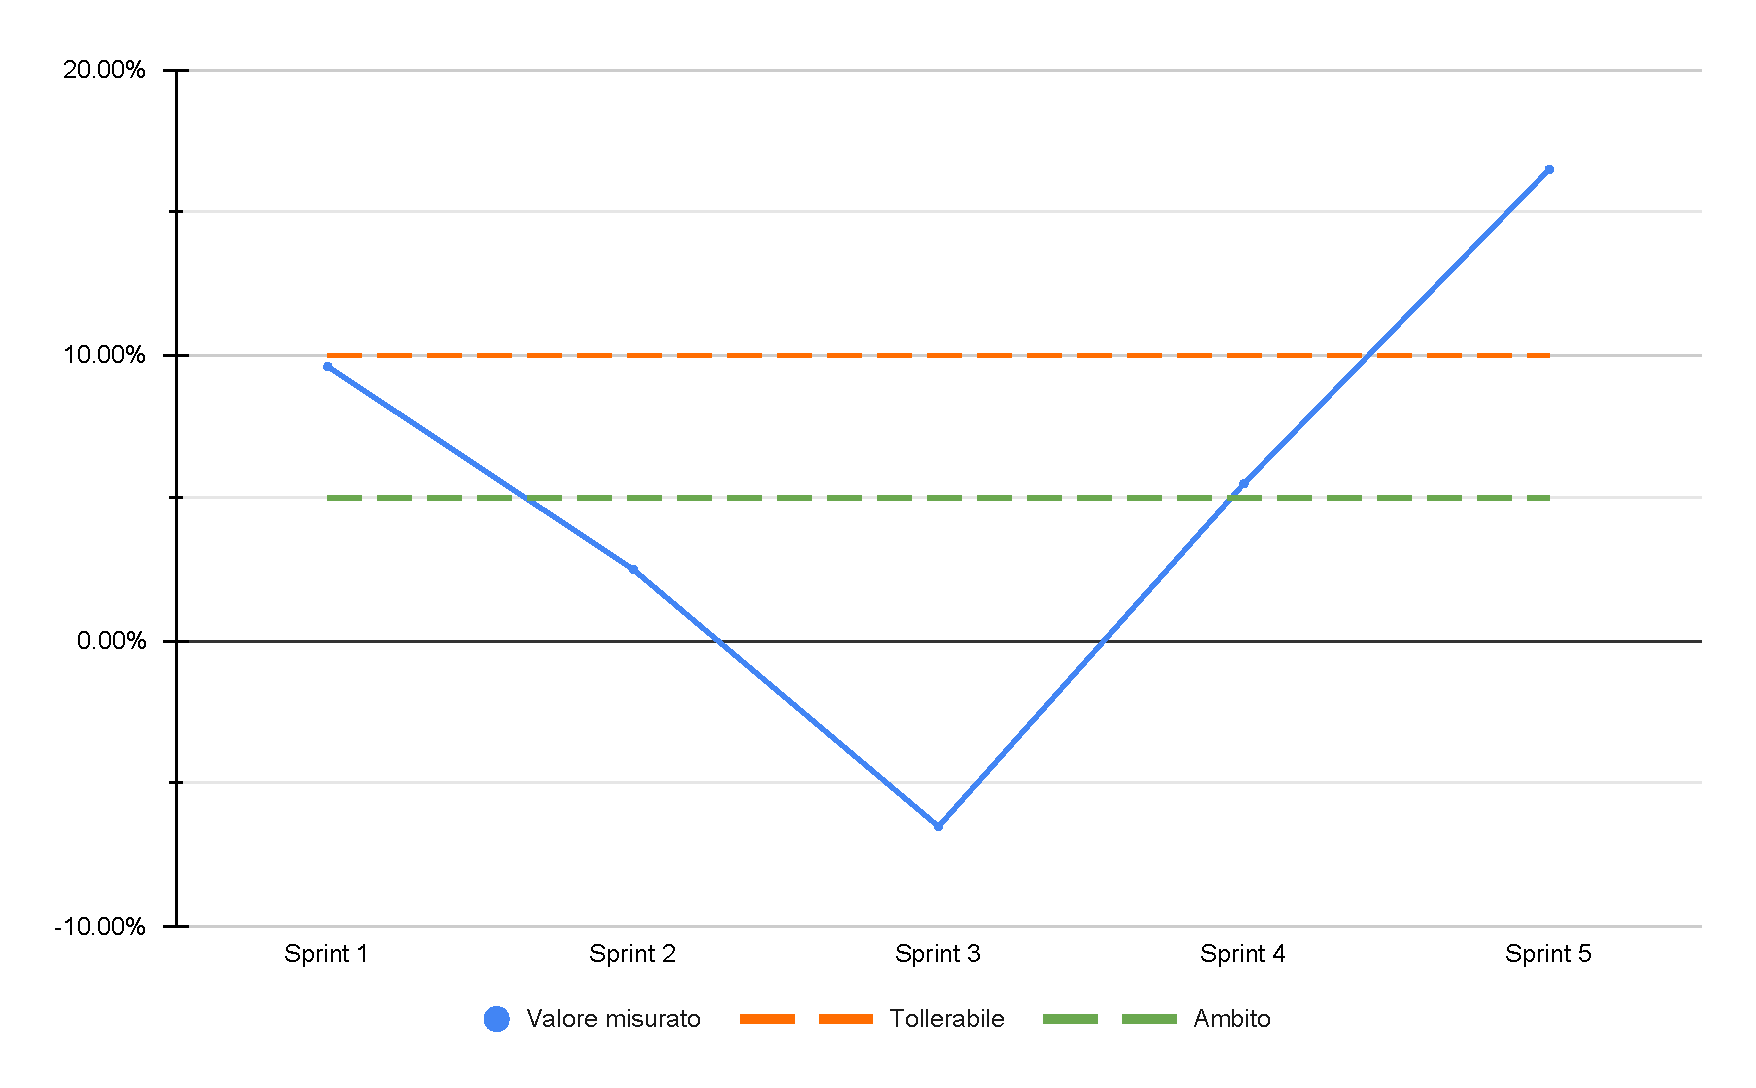
\includegraphics[width=0.8\textwidth]{assets/variazione_costo.pdf}
    \caption{M.2.3 Variazione di costo}
\end{figure}

\par Il grafico mostra come dal primo \glossario{sprint}, il gruppo abbia lavorato rispettando i costi proposti sul preventivo per lo \glossario{sprint}. Questo è visto sia in termini positivi che negativi, poiché una variazione di costo vicina alla soglia di tollerabilità, è anche indice di inesperienza sulla distribuzione dei ruoli e sulla gestione delle attività o di criticità che hanno rallentato i lavori, aumentando il costo complessivo dello \glossario{sprint}.
Durante gli \glossario{sprint} successivi, il gruppo ha lavorato in modo più efficiente, avvicinandosi sempre di più al costo preventivato. Dallo \glossario{sprint} 4, il grafico ha una nuova risalita dovuta ad un cambio di tecnologie che ha comportato un aumento dei costi al di sopra della soglia tollerabile. La tendenza generale del grafico, dal secondo \glossario{sprint} è comunque sempre rimasta compresa tra il valore ambito e il valore tollerabile. 
\clearpage
\subsection{M.PC.9 - Frequenza di merge delle pull request}
\begin{figure}[H]
    \centering
    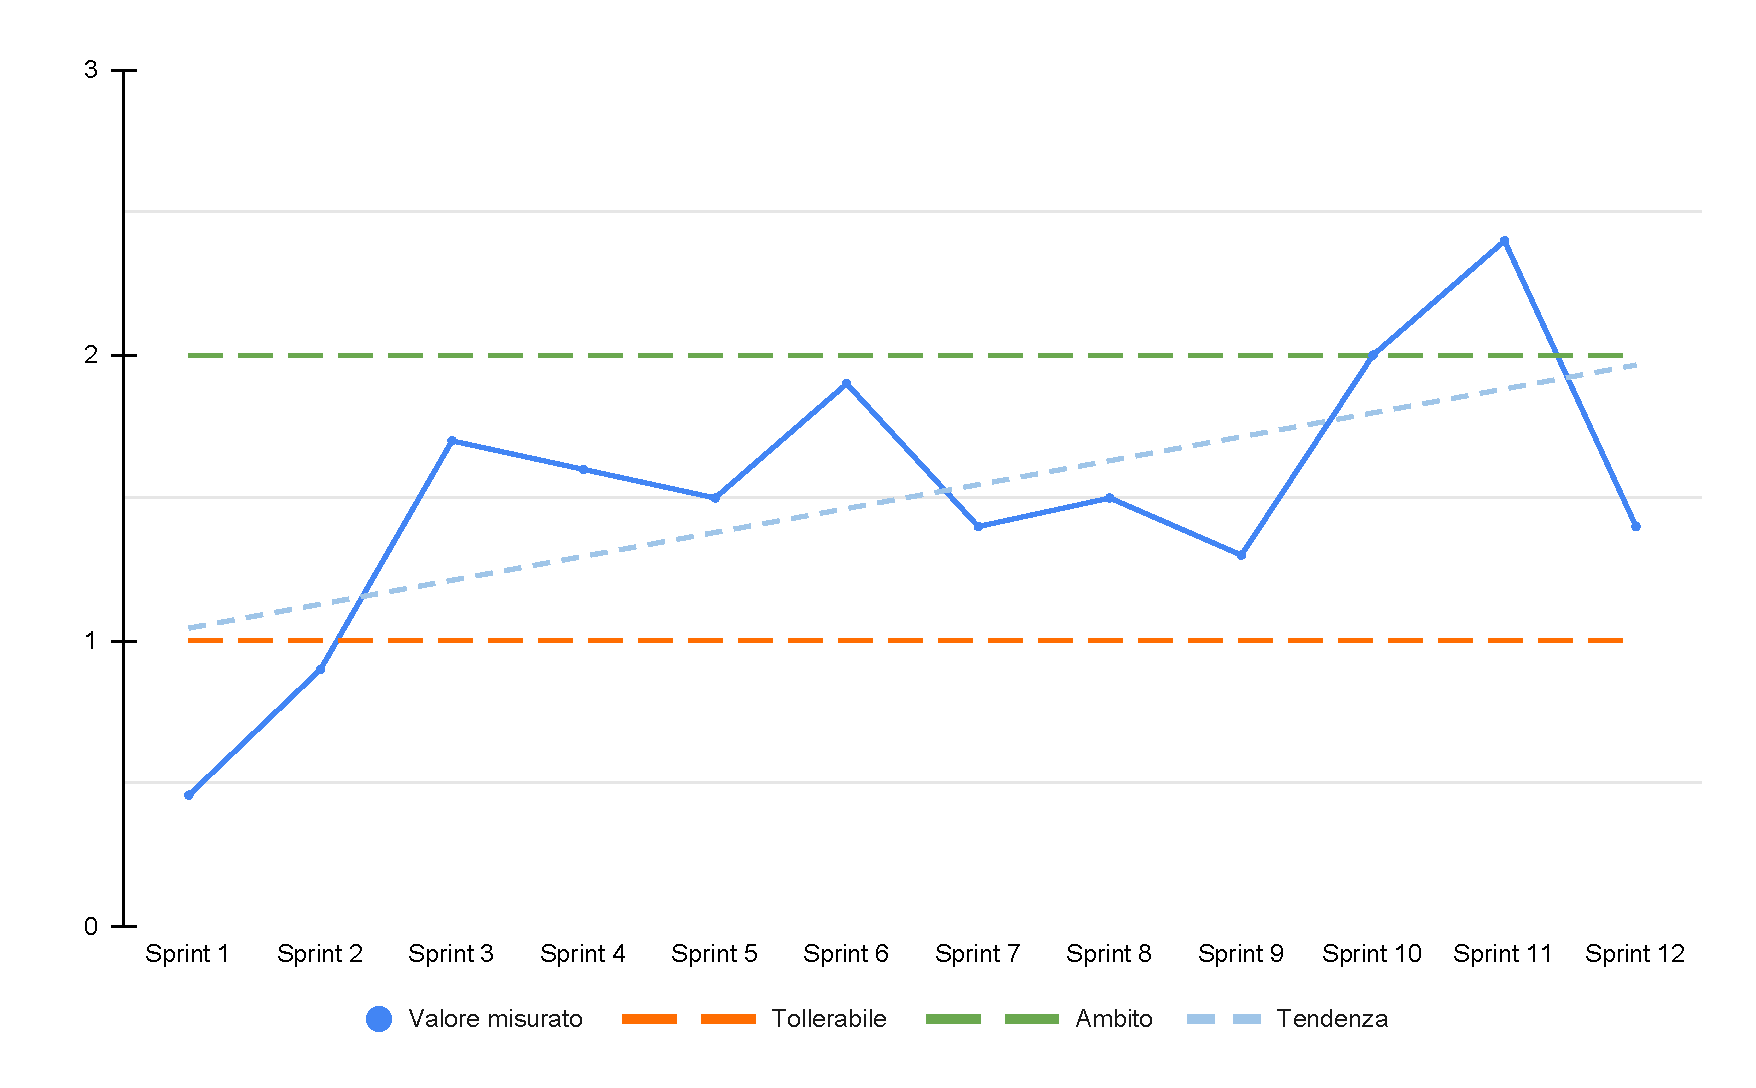
\includegraphics[width=\textwidth]{assets/frequenza_pull_request.pdf}
    \caption{M.PC.9 - Frequenza di merge delle pull request}
\end{figure}

\par Nei primi due \glossario{sprint}, la frequenza di merge delle pull request è stata inferiore alle aspettative; questo è dovuto al fatto che, nelle fasi iniziali del progetto, gli sforzi del gruppo si sono concentrati sulla produzione di documenti. Data l'inesperienza del team nella stesura della documentazione, le pull request sono state aperte con discontinuità. Inoltre, la portata delle modifiche ha rallentato il processo di verifica e approvazione. Pertanto, la frequenza di merge non ha raggiunto il valore tollerabile (1 volta al giorno). Il team ha quindi deciso di ridurre il valore ambito, da 3 volte al giorno a 2. Dal terzo sprint, vista la necessità di aggiornare specifiche sezioni dei documenti, il gruppo ha ritenuto opportuno integrare le modifiche con maggior frequenza. È stata introdotta la pratica di \glossario{continuous integration}, migliorando il processo di allineamento delle modifiche e consentendo verifiche rapide e frequenti. Un fattore che ha contribuito a incrementare la frequenza di merge è stato lo sviluppo del \glossario{PoC}, le cui funzionalità sono state suddivise in task di dimensioni ridotte, al fine di promuovere l'integrazione continua. Grazie all'applicazione di questa contromisura, il team ha mantenuto un flusso di lavoro regolare. Come testimonia il grafico, i valori misurati a partire dal terzo sprint rientrano nel range di tollerabilità stabilito. In concomitanza del sesto sprint, la frequenza di merge delle pull request si è avvicinata al valore ambito; considerando il cambio di tecnologie avvenuto nell'iterazione precedente, questo risultato dimostra l'efficacia delle strategie adottate dal gruppo.

\par Nella prima fase della \glossario{PB}, la frequenza di merge delle pull request ha raggiunto la soglia ambita. Questo risultato è in linea con la decisione del team di applicare con maggior rigore la pratica di \glossario{integrazione continua}. Nel dodicesimo sprint, invece, il valore misurato è rimasto al di sotto della soglia ambita, poiché l'integrazione delle modifiche (tramite il meccanismo delle pull request) ha richiesto più tempo del previsto. Nonostante ciò, la frequenza di merge è rimasta entro i limiti di tollerabilità.

\clearpage
\subsection{M.PC.11 - Rischi inattesi}
\begin{figure}[H]
    \centering
    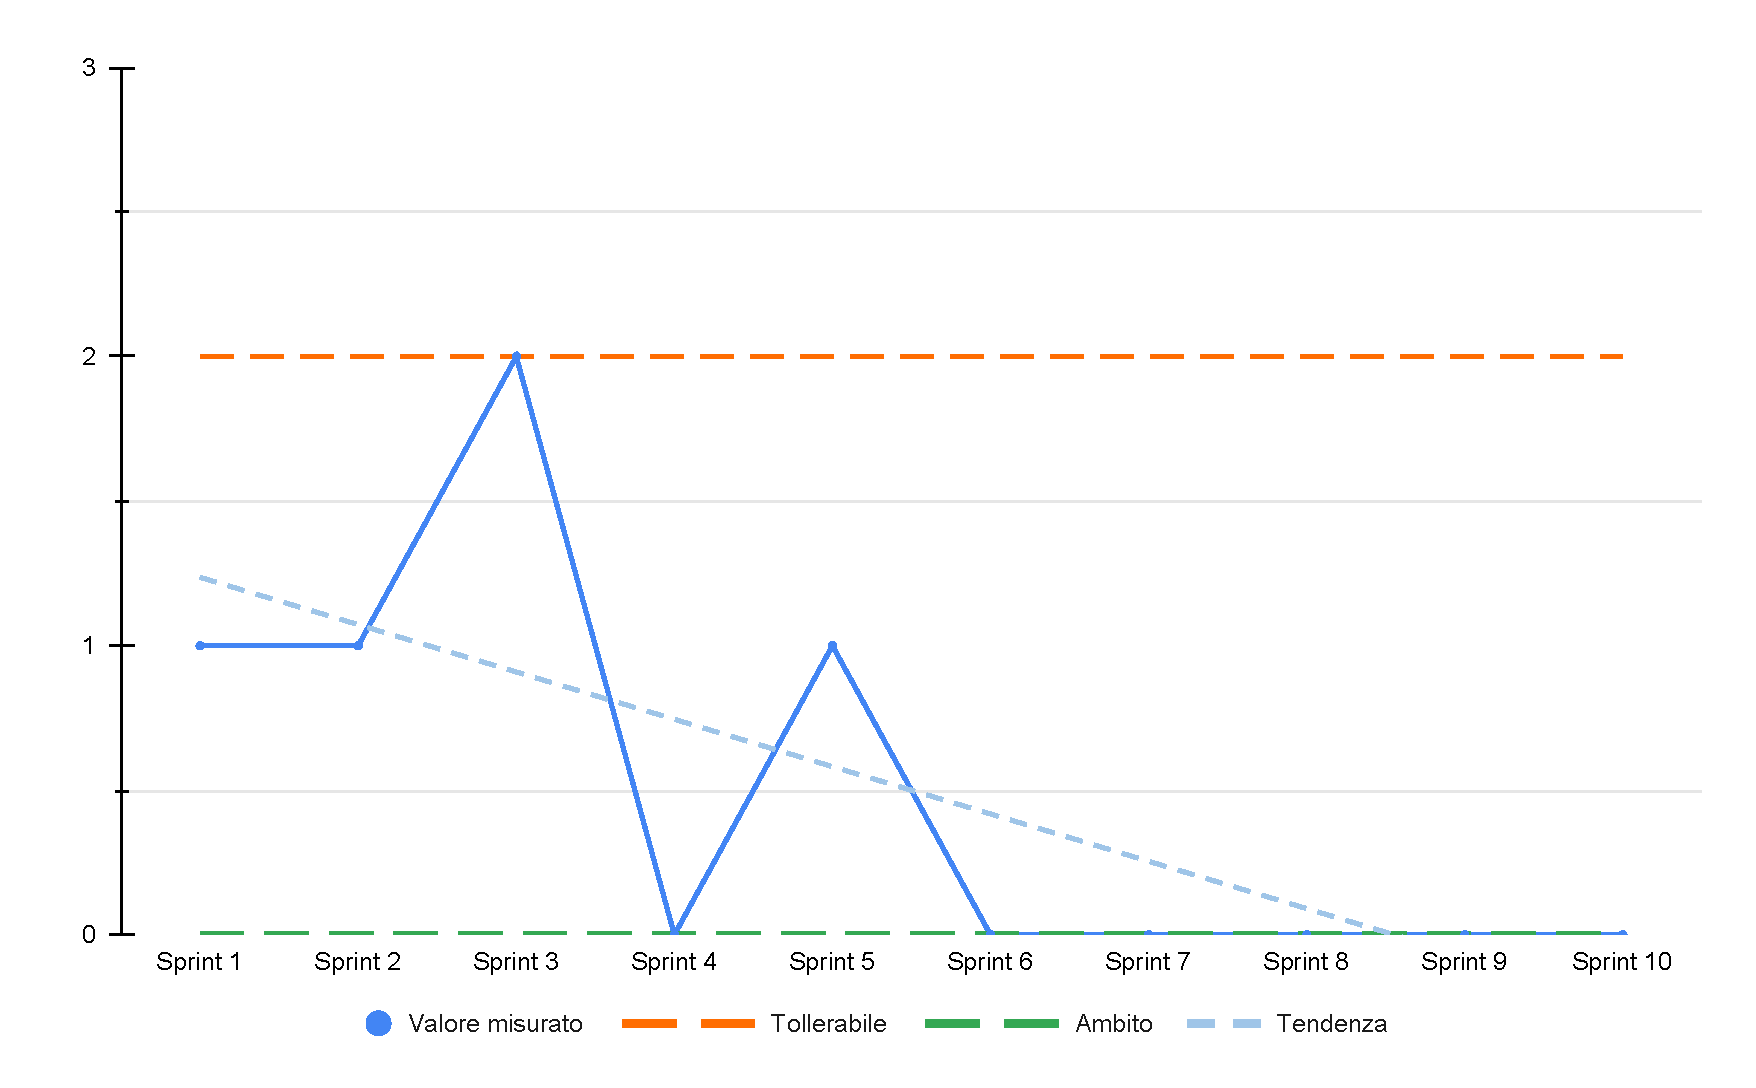
\includegraphics[width=\textwidth]{assets/rischi_inattesi.pdf}
    \caption{M.PC.11 - Rischi inattesi}
\end{figure}

\par Il grafico evidenzia l’inesperienza iniziale del team nell’individuare i rischi che possono emergere durante lo svolgimento di un progetto software. Nei primi tre \glossario{sprint}, infatti, il gruppo ha dovuto affrontare almeno un rischio inatteso. Ciononostante, il numero di rischi imprevisti è rimasto entro i limiti della soglia tollerabile. A partire dal quarto sprint, i rischi che si sono verificati erano già stati analizzati e documentati nel \PdP. Attraverso un’analisi più consapevole, una collaborazione stretta tra i membri e una comunicazione trasparente, il team ha mantenuto il numero di eventi imprevisti stabile e prossimo al valore ambito. L'unica eccezione è stata il sesto sprint, durante il quale è emerso un rischio inatteso legato al cambio di tecnologie. Nonostante il gruppo avesse previsto una possibile transizione e avesse testato diversi \glossario{framework} alternativi, l’entità del lavoro risultante ha superato le risorse disponibili, prolungando le scadenze prefissate. Per migliorare la gestione del progetto, il gruppo ha convenuto di discutere e monitorare i rischi durante le riunioni interne, fornendo al responsabile una base solida per la stesura del \PdP. L'obiettivo per le iterazioni successive è di ridurre il valore tollerabile a 1, mantenendo una gestione stabile dei rischi.

\clearpage
\input{valutazionemetriche/stabilità_requisiti}
\clearpage

\end{document}